% !TEX root = ../my-thesis.tex

\graphicspath{{./content/chap4_econobiology/figures/}}

\clearpage
\section{Supplementary Figures}

\begin{figure}[ht]
  \center
  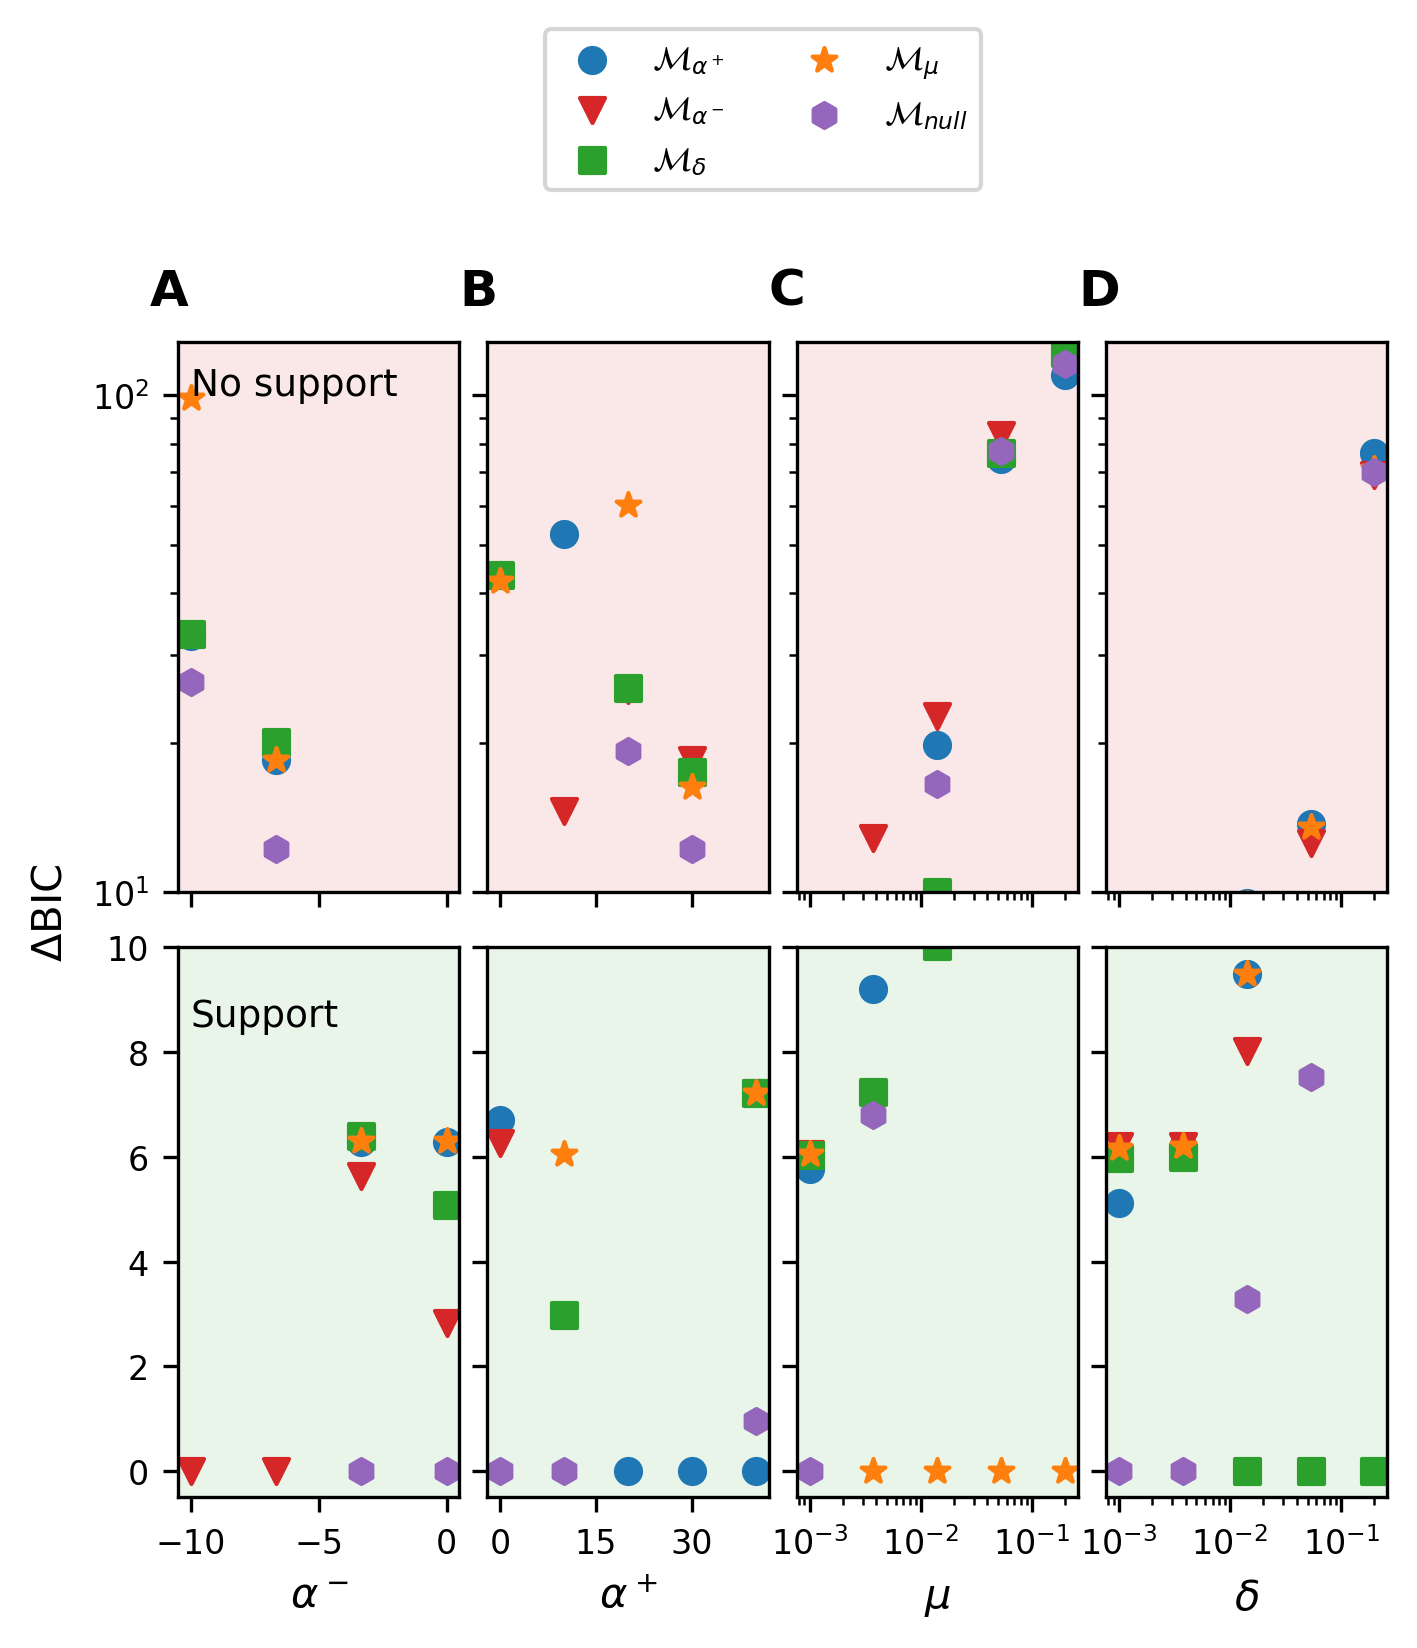
\includegraphics{SI/synthetic_test_all_AIC_r=0.3.png}
  \caption{\small \textbf{Validation of the model selection procedure}. The figure is analogous to \cref{fig:synthetic_test_all_AIC} but with $\sigma = 0.3$. 
   }\label{figSI:synthetic_test_all_AIC}
\end{figure}

\begin{figure}[ht]
  \center
  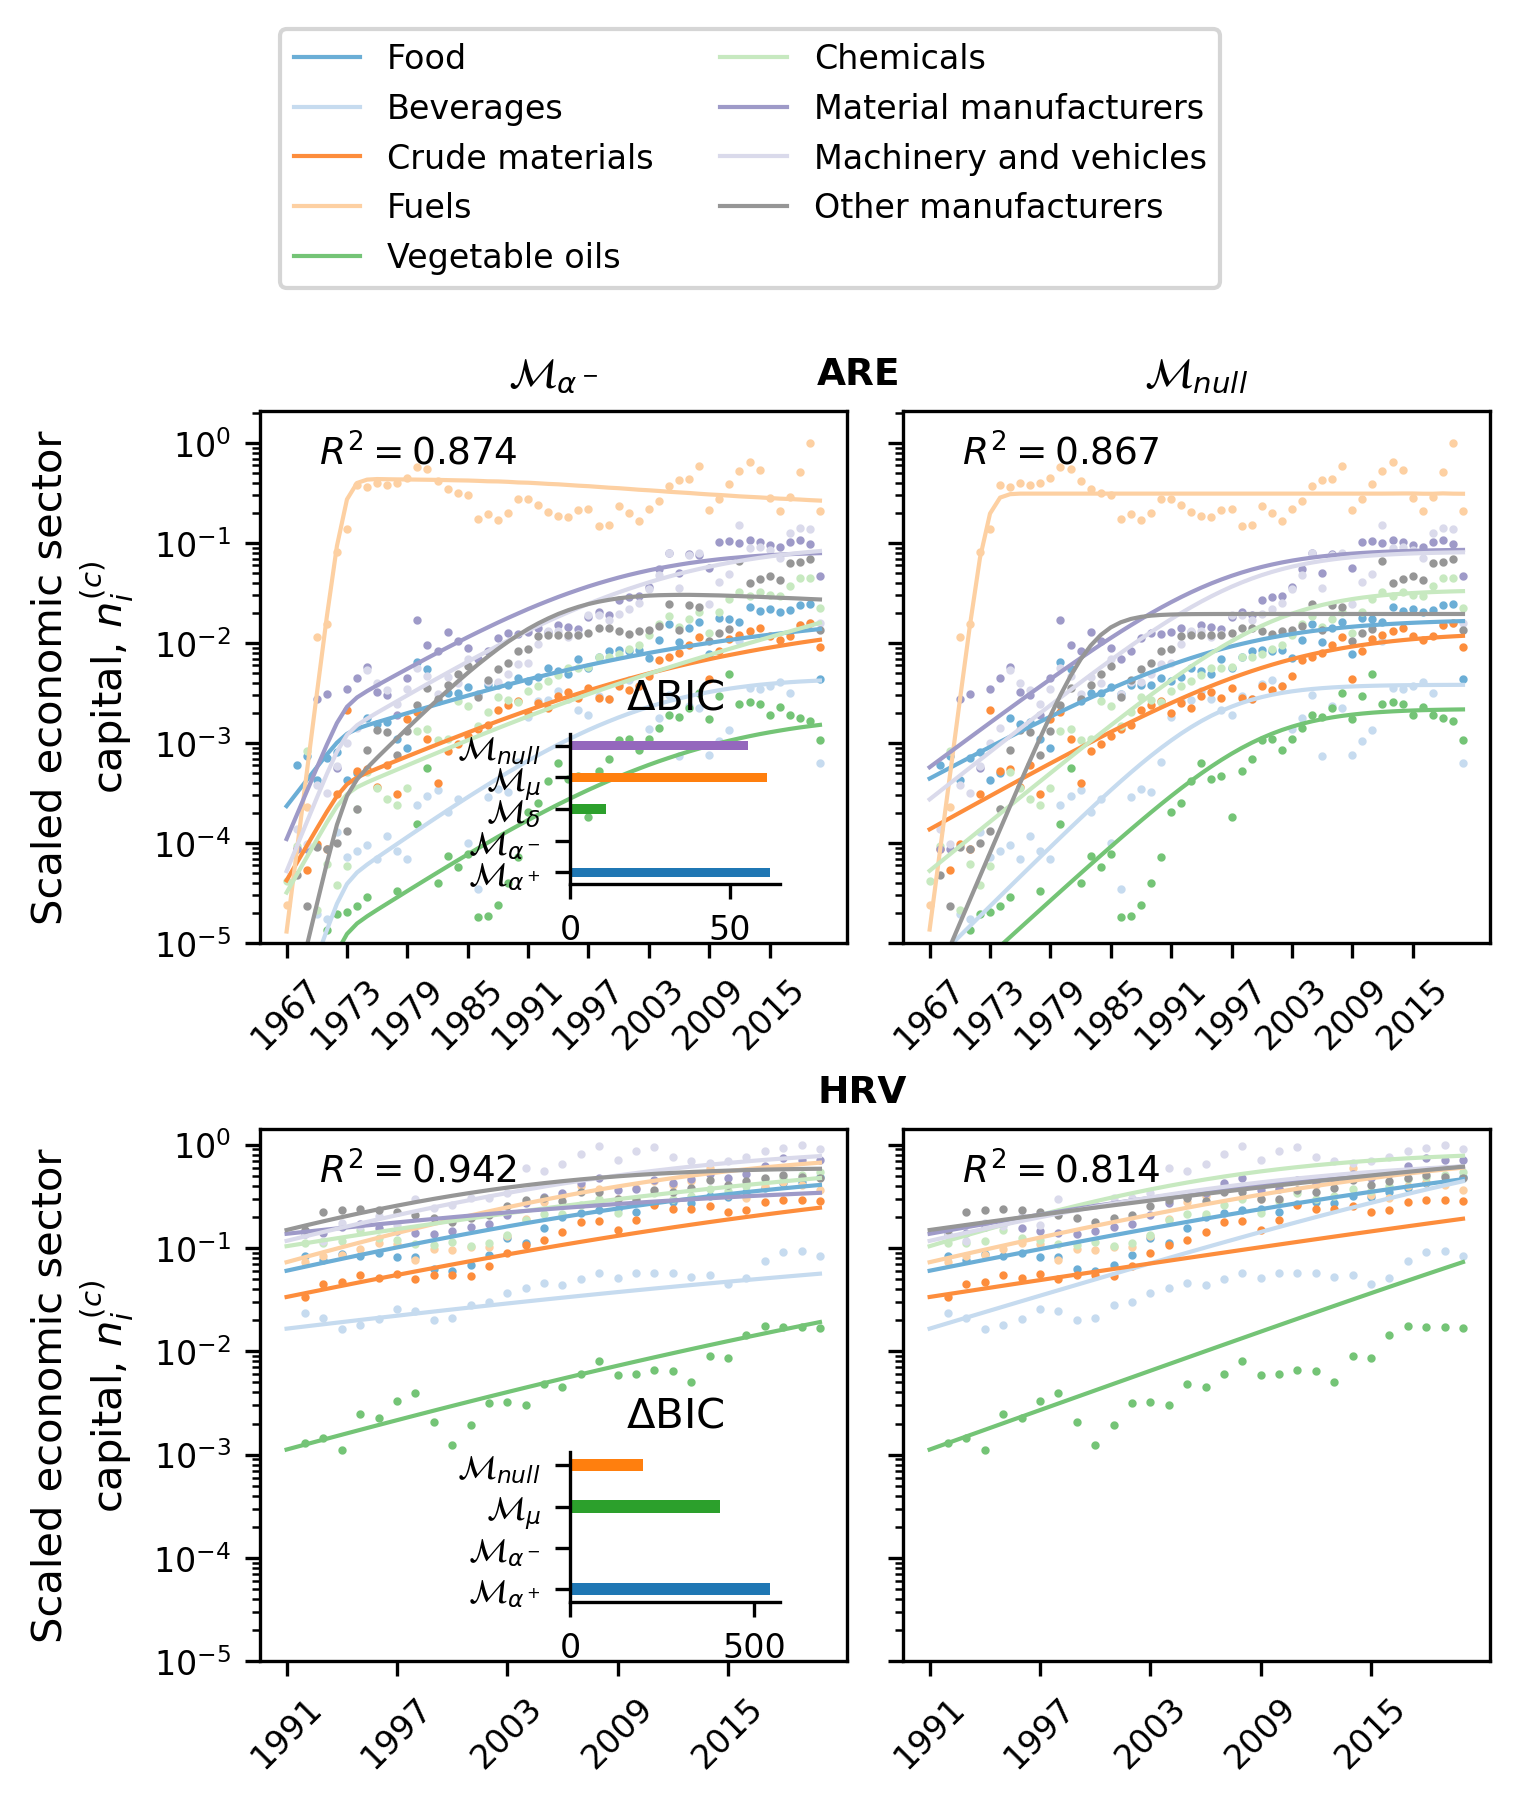
\includegraphics{SI/figure_alphan_simulate.png}
  \caption{\small \textbf{Fits of model $\modalphan$ for ARE and HRV, where $\modalphan$ is given support against $\modnull$}. 
   }\label{figSI:fit_alphan}
\end{figure}

\begin{figure}[ht]
  \center
  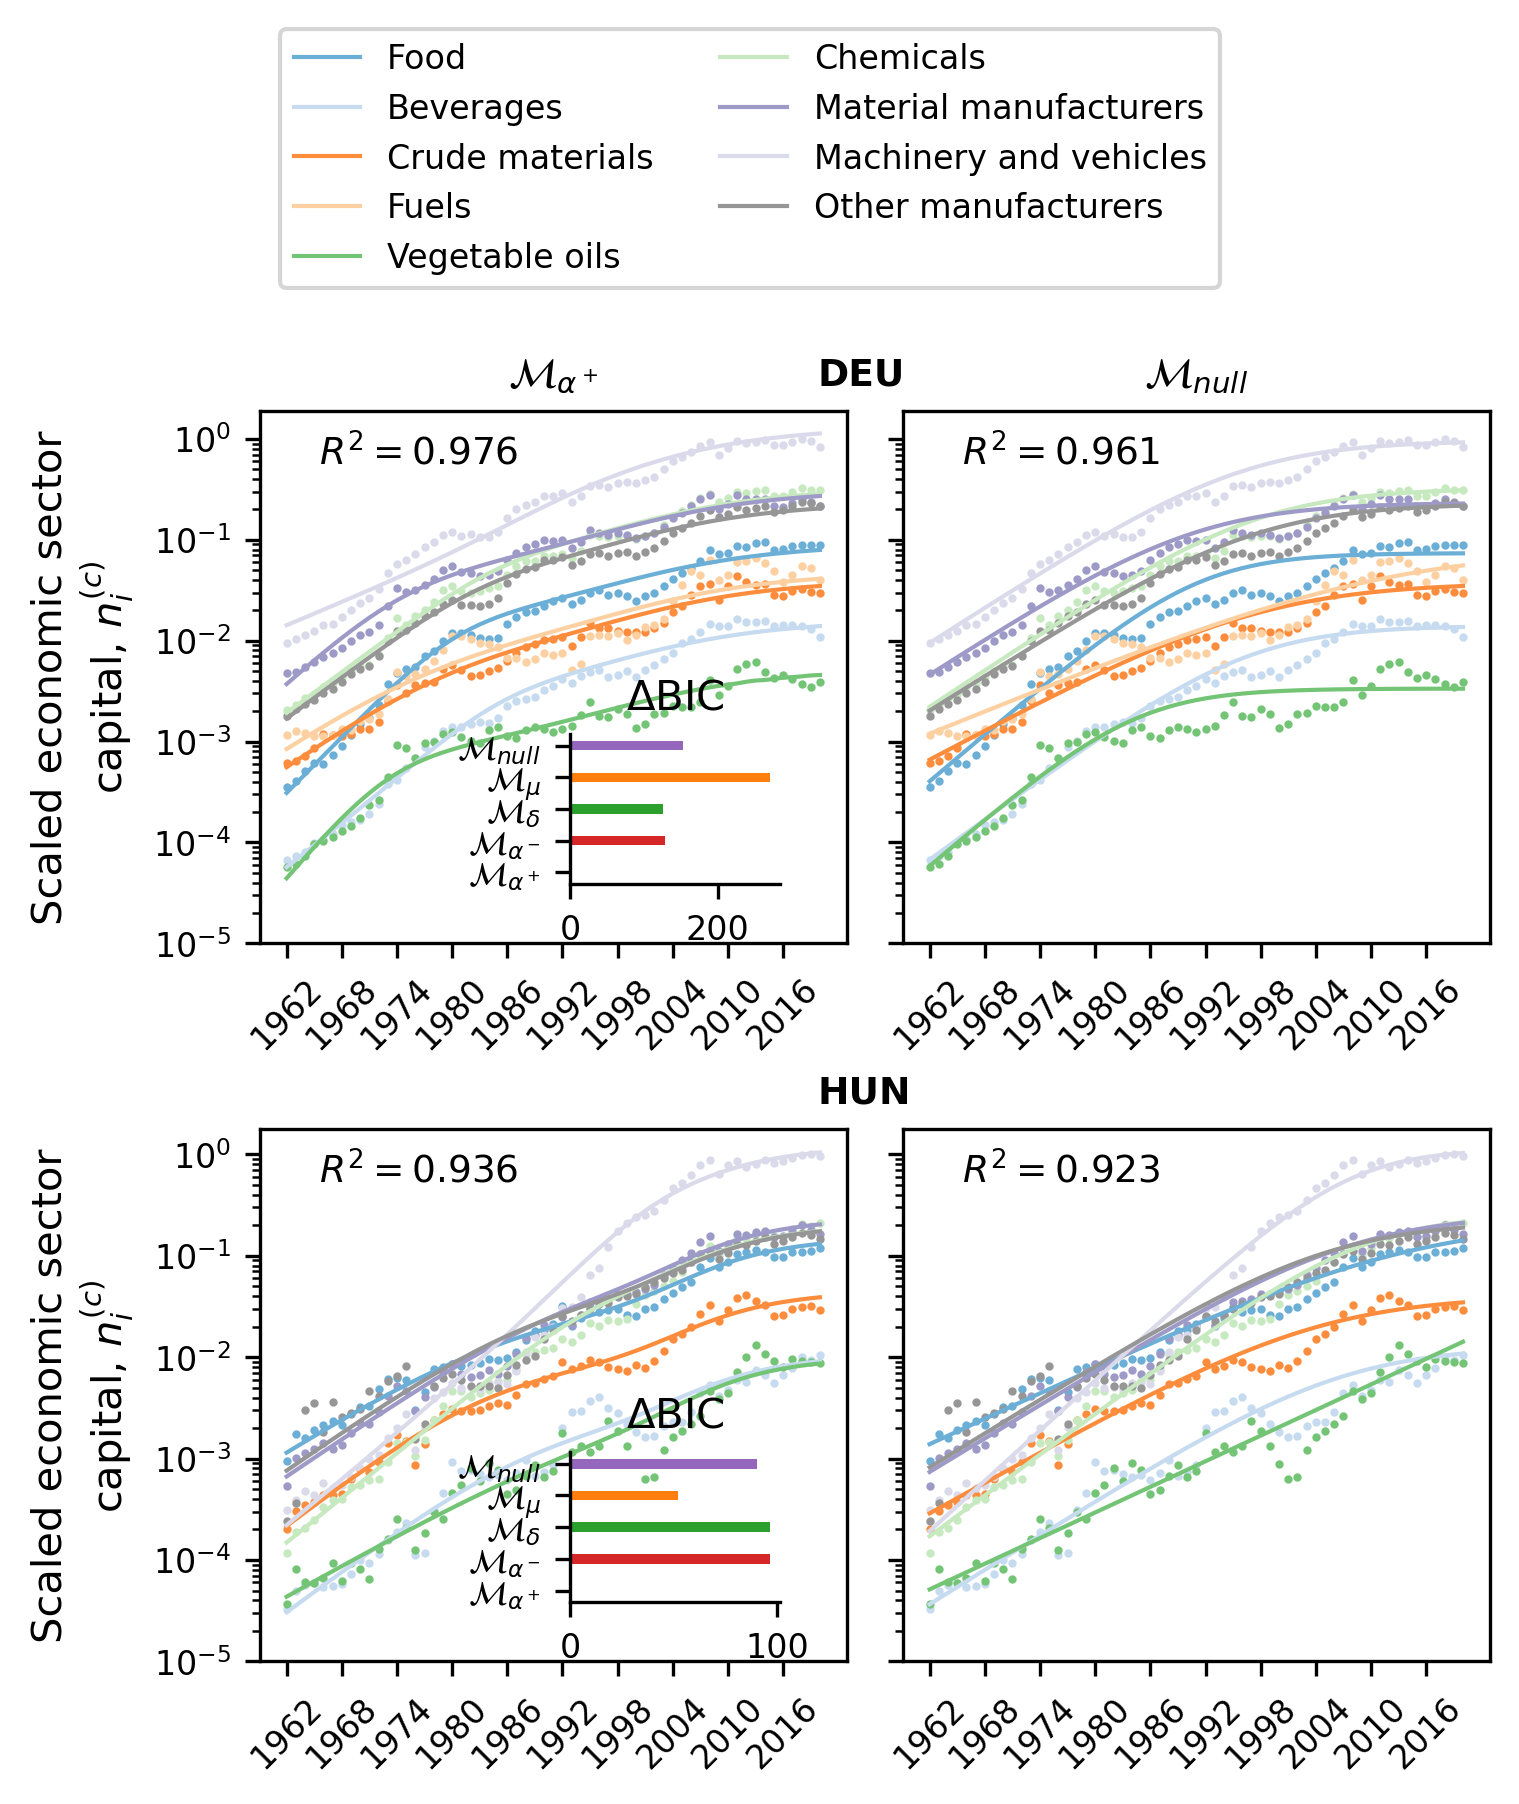
\includegraphics{SI/figure_alphap_simulate.png}
  \caption{\small \textbf{Fits of model $\modalphap$ for DEU and HUN, where $\modalphap$ is given support against $\modnull$}. 
   }\label{figSI:fit_alphap}
\end{figure}

\begin{figure}[ht]
  \center
  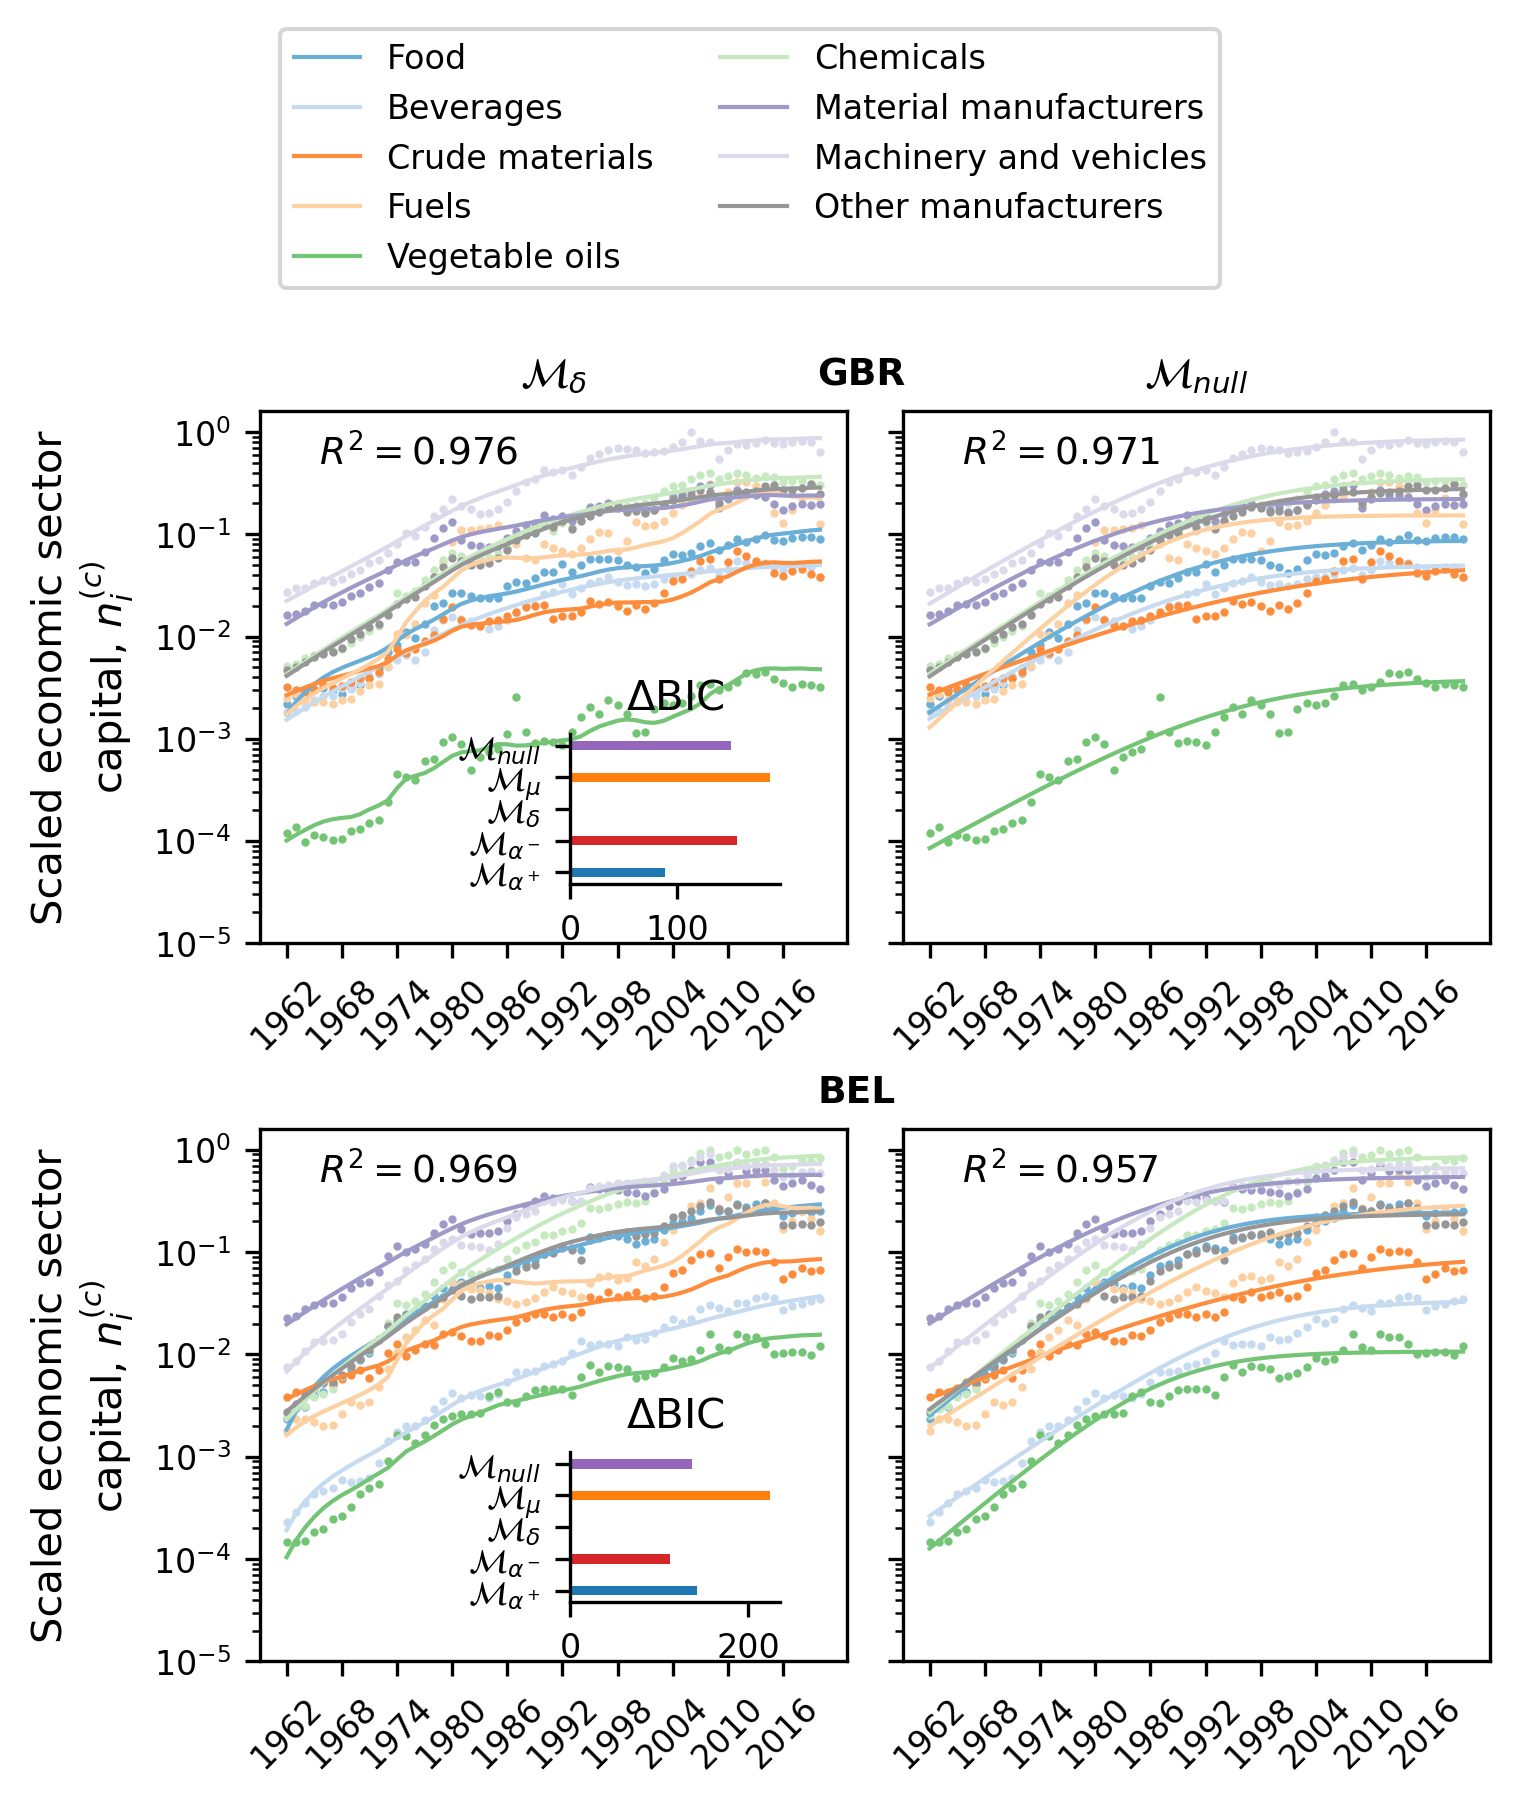
\includegraphics{SI/figure_delta_simulate.png}
  \caption{\small \textbf{Fits of model $\moddelta$ for GBR and BEL, where $\moddelta$ is given support against $\modnull$}. 
   }\label{figSI:fit_delta}
\end{figure}

\begin{figure}[ht]
  \center
  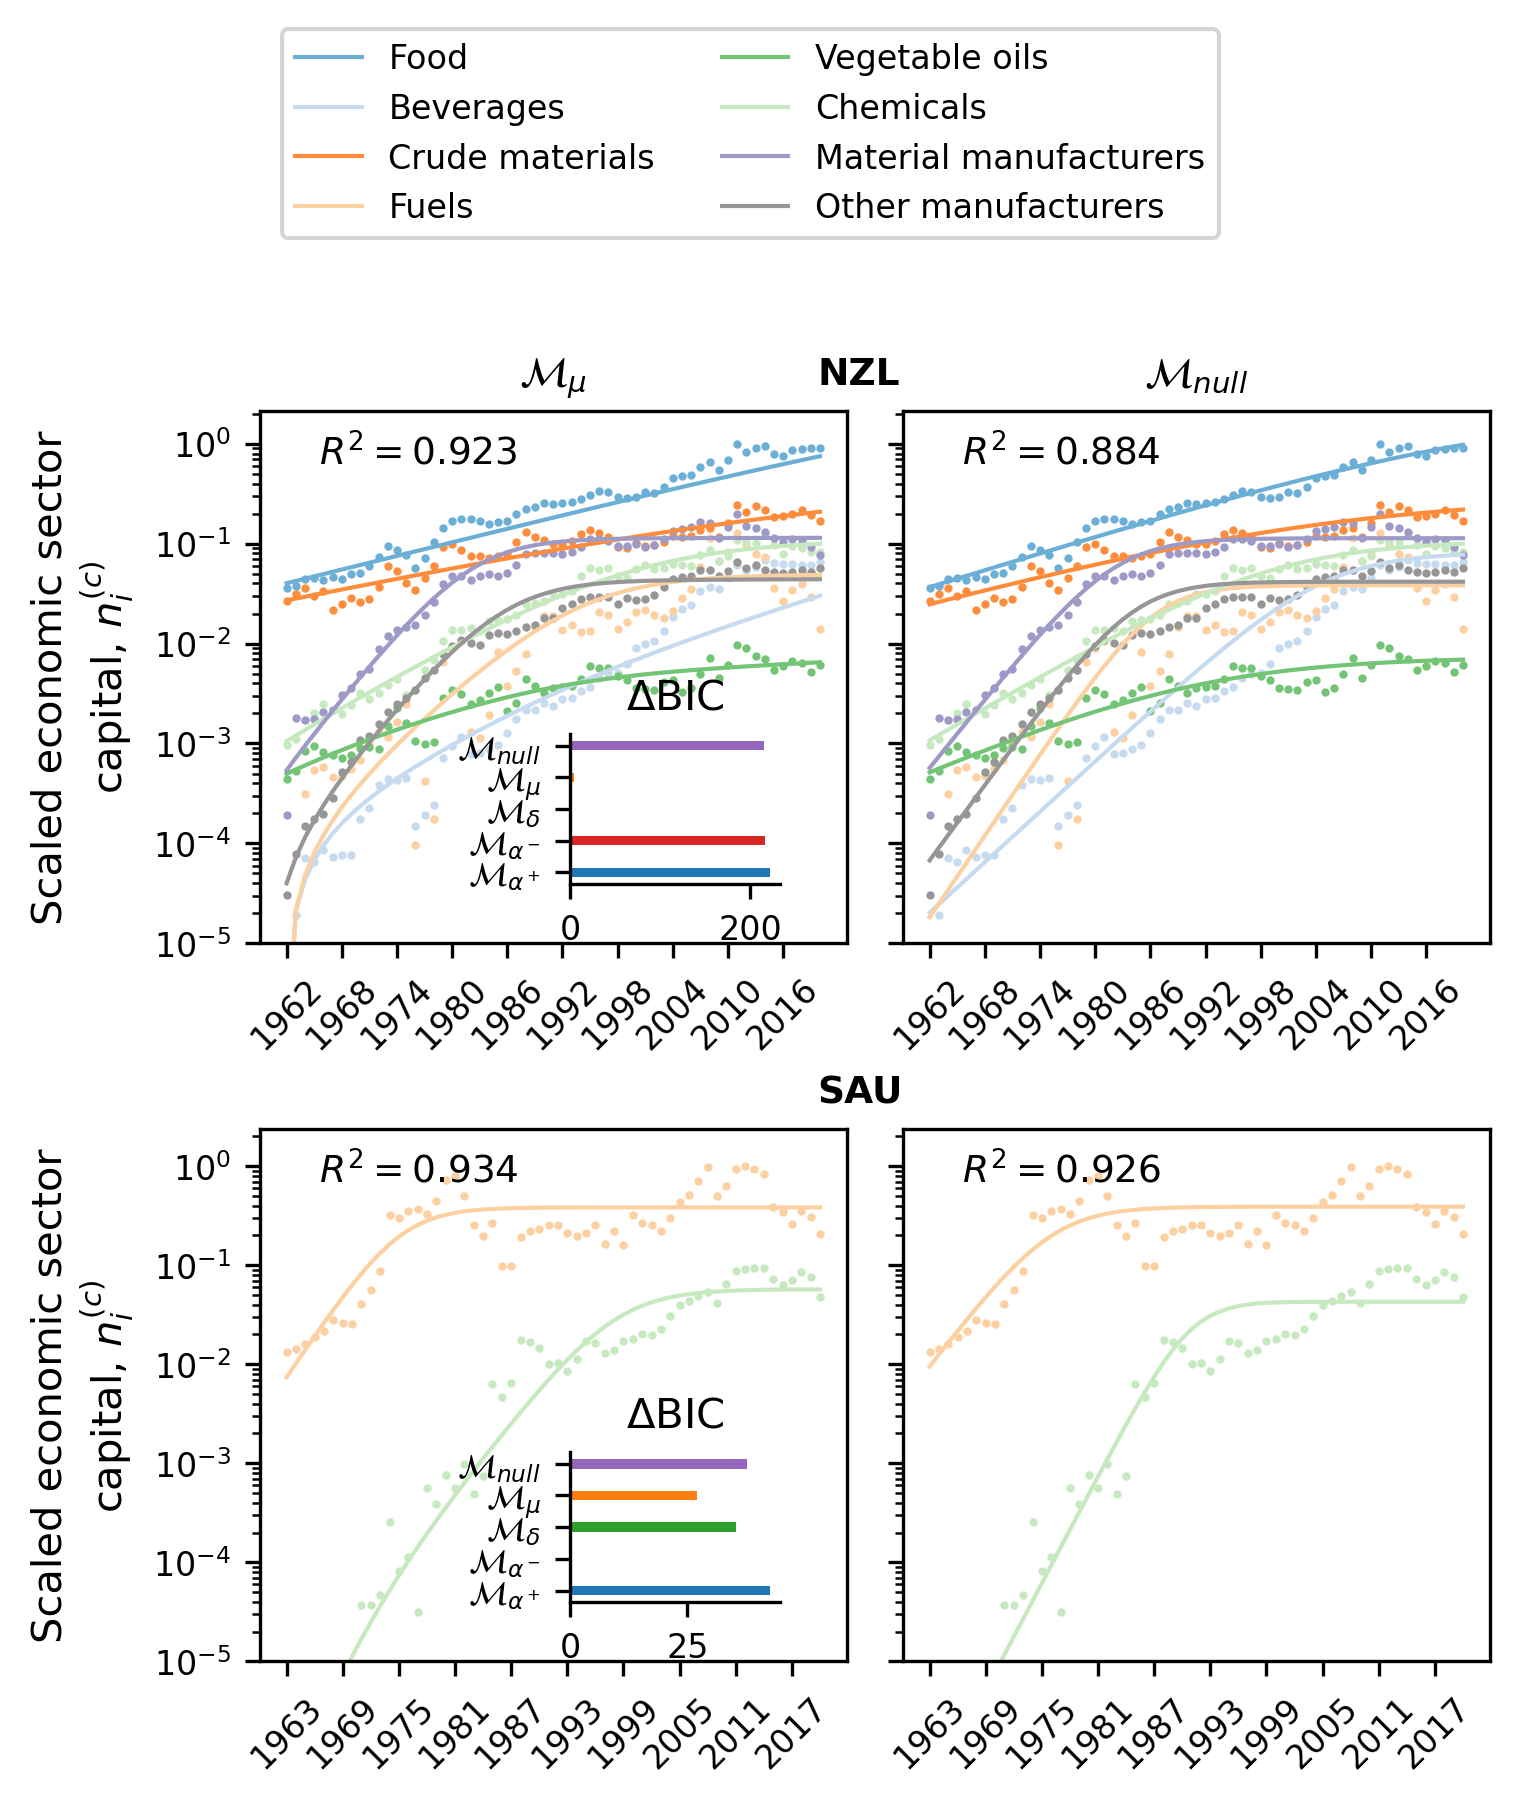
\includegraphics{SI/figure_mu_simulate.png}
  \caption{\small \textbf{Fits of model $\modmu$ for NZL and KOR, where $\modmu$ is given support against $\modnull$}. 
   }\label{figSI:fit_mu}
\end{figure}

\begin{figure}[ht]
  \center
  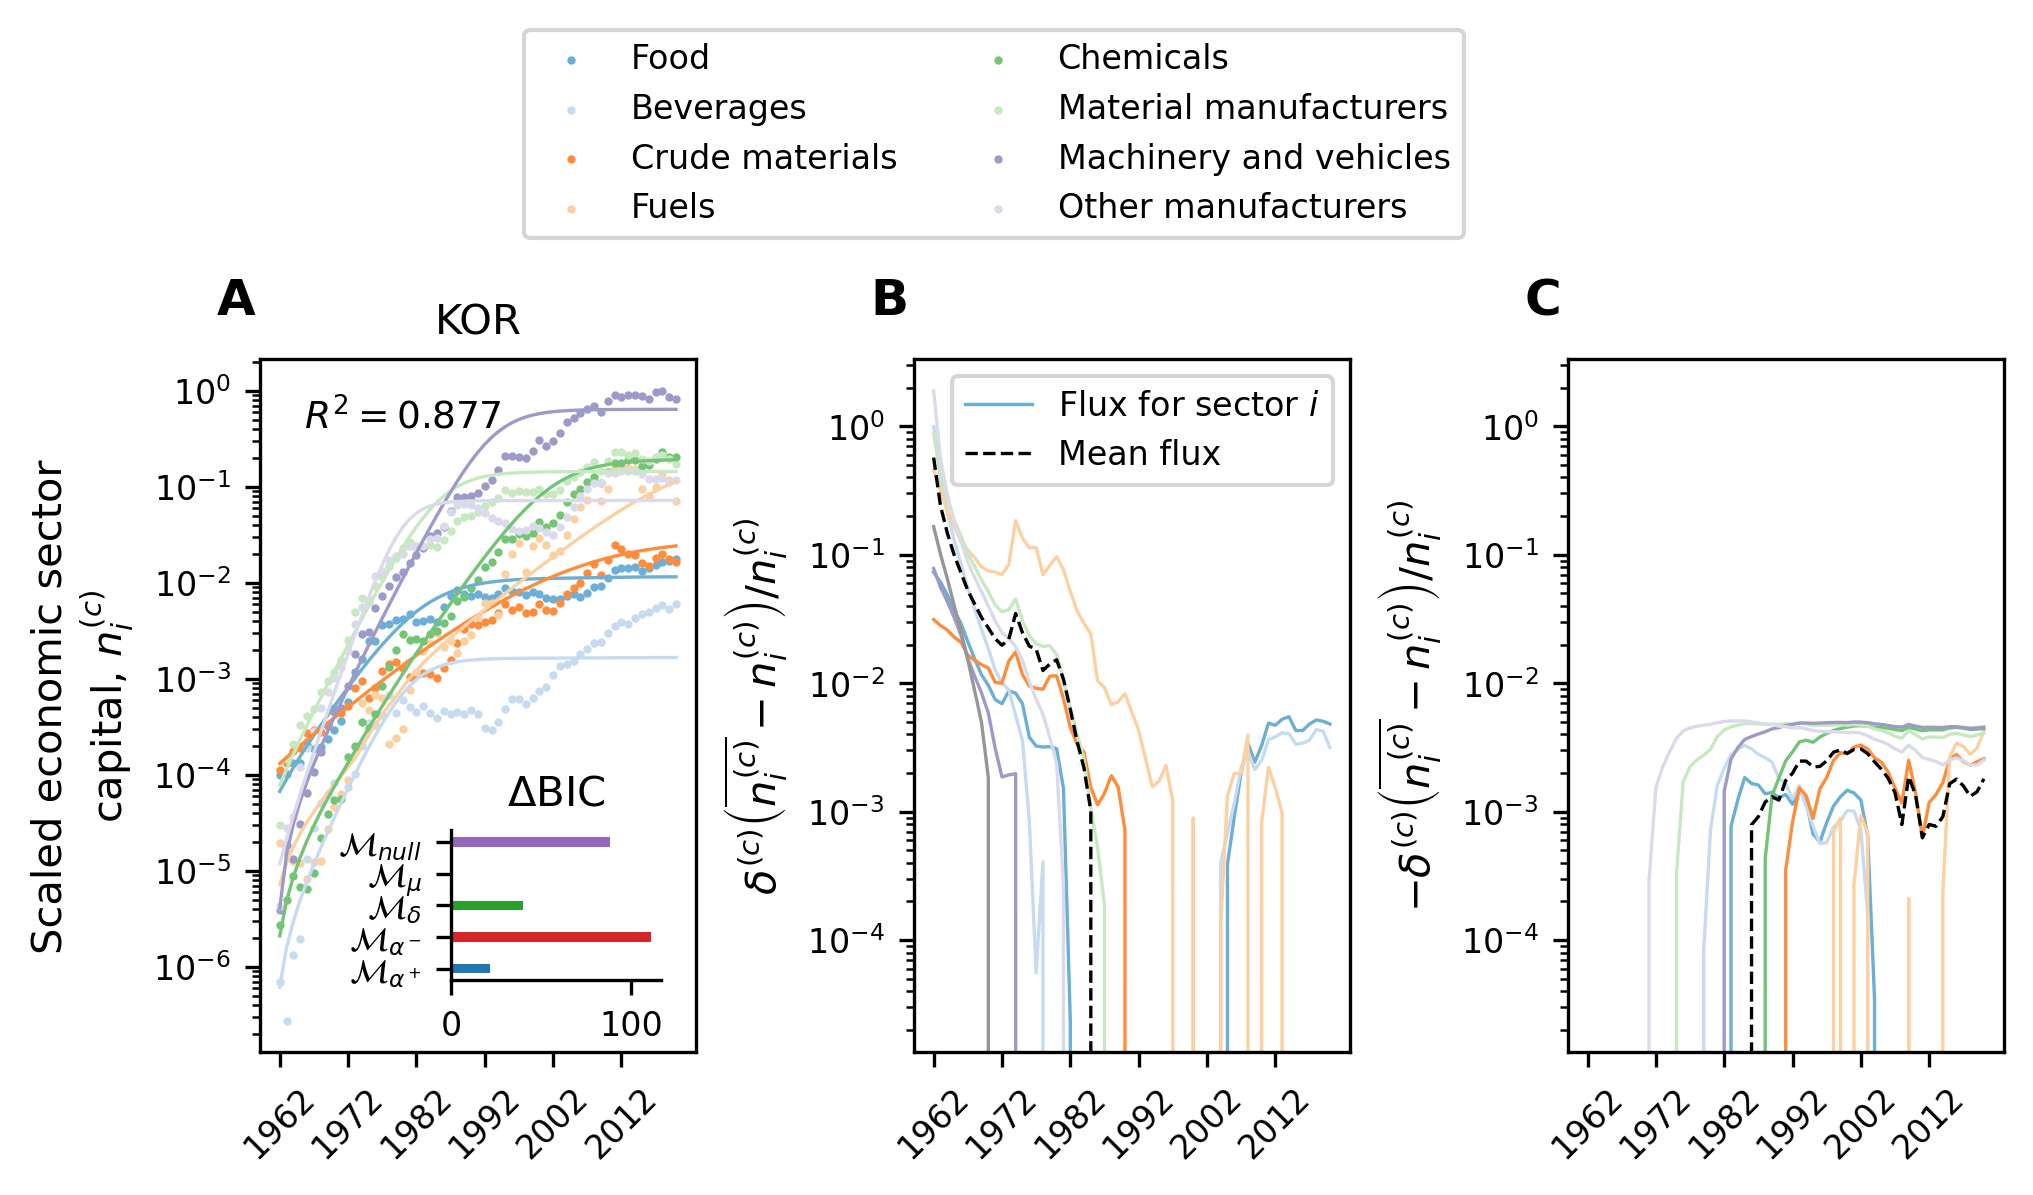
\includegraphics{SI/flux_delta.png}
  \caption{\small \textbf{Contributions of fluxes due to spatial dispersal on growth dynamics}. \textbf{A} shows the growth dynamics for KOR, together with the best model fit. \textbf{B}-\textbf{C} show the positive and negative fluxes, respectively, due to spatial dispersal for each economic activity, relative to the capital size of economic activity. The contributions of spatial dispersal to growth decreases over time.
  }\label{figSI:flux_delta}
\end{figure}

\clearpage 

\section{Supplementary Tables}

\begin{table}[ht]
    \begin{center}
      \begin{scriptsize}
\pgfplotstabletypeset[
columns={Country Code, Country Name, Country Code, Country Name},
display columns/0/.style={select equal part entry of={0}{2},string type},% first part of ‘A’
display columns/1/.style={select equal part entry of={0}{2},string type},% first part of ‘B’
display columns/2/.style={select equal part entry of={1}{2},string type},% second part of ‘A’
display columns/3/.style={select equal part entry of={1}{2},string type},% second part of ‘B’
]{\datatable}
\end{scriptsize}

    \end{center}
    \caption{\textbf{ISO 3166-1 country codes for each of the 100 country investigated.}}
    \label{tab:country_codes}
\end{table}

% \begin{footnotesize}
\setlength\LTcapwidth{\linewidth}
\begin{longtable}[ht]{|c|c|c|c|c|c|c|}
    \hline
        Country & Model & Loss & Rel. std. loss & R2 & Log-likelihood & $\Delta \text{BIC}$\\
    \hline
    \endhead
    % \hline
    \endfoot
    \hline

    \caption{\textbf{Results of the numerical simulations}. Numerical values for each model and each country correspond to the optimization run with the minimum loss value. "Rel. std. loss" corresponds to the standard deviation of the loss values obtained for the five independent runs, divided by the mean loss value. Low "Rel. std. loss" indicates that the optimization runs have converged towards the same maximum likelihood.}
    \label{tab:results}
    \endlastfoot
    ARE & $\mathcal{M}_{\alpha^+}$ & 1.2527837 & 0.0443378 & 0.8985771 & 2194.9947804 & -331.4965062\\
ARE & $\mathcal{M}_{\alpha^-}$ & 1.1323544 & 0.0001987 & 0.9070505 & 2209.3385519 & -374.6811568\\
ARE & $\mathcal{M}_{\delta}$ & 1.1547997 & 0.0018924 & 0.9037398 & 2204.4213038 & -357.3571273\\
ARE & $\mathcal{M}_{\mu}$ & 1.3237895 & 0.0096762 & 0.8908284 & 2175.1338748 & -295.0532417\\
ARE & $\mathcal{M}_{null}$ & 1.3210473 & 0.0185026 & 0.8945233 & 2184.4961044 & -318.3014521\\
ARG & $\mathcal{M}_{\alpha^+}$ & 0.5362716 & 0.0000000 & 0.9126885 & 873.2783542 & -479.0901860\\
ARG & $\mathcal{M}_{\alpha^-}$ & 0.5260177 & 0.0000000 & 0.9148312 & 877.0708569 & -486.6684522\\
ARG & $\mathcal{M}_{\delta}$ & 0.5347459 & 0.0882225 & 0.9127092 & 873.5096285 & -479.1622984\\
ARG & $\mathcal{M}_{\mu}$ & 0.5362716 & 0.0000000 & 0.9126884 & 873.2790114 & -479.0898098\\
ARG & $\mathcal{M}_{null}$ & 0.5362716 & 0.0000000 & 0.9126885 & 873.2797678 & -484.8104788\\
AUS & $\mathcal{M}_{\alpha^+}$ & 0.2493686 & 0.0259488 & 0.9701803 & 1746.6372258 & -1152.0686387\\
AUS & $\mathcal{M}_{\alpha^-}$ & 0.2639190 & 0.0000105 & 0.9687099 & 1734.9134560 & -1128.5804718\\
AUS & $\mathcal{M}_{\delta}$ & 0.3009456 & 0.0013734 & 0.9620972 & 1683.0297057 & -1035.0200199\\
AUS & $\mathcal{M}_{\mu}$ & 0.2639179 & 0.0000000 & 0.9687119 & 1734.9252830 & -1128.6123545\\
AUS & $\mathcal{M}_{null}$ & 0.2639178 & 0.0000001 & 0.9687114 & 1734.9245624 & -1134.7946683\\
AUT & $\mathcal{M}_{\alpha^+}$ & 0.2068390 & 0.0001061 & 0.9818722 & 2225.2530696 & -1414.8850719\\
AUT & $\mathcal{M}_{\alpha^-}$ & 0.1927354 & 0.0000609 & 0.9831719 & 2245.3364190 & -1455.7289956\\
AUT & $\mathcal{M}_{\delta}$ & 0.1858071 & 0.0000049 & 0.9836237 & 2253.3349649 & -1470.6709565\\
AUT & $\mathcal{M}_{\mu}$ & 0.1967636 & 0.0000009 & 0.9827050 & 2238.1320372 & -1440.7057723\\
AUT & $\mathcal{M}_{null}$ & 0.2068390 & 0.0000001 & 0.9818725 & 2225.2566207 & -1421.2047025\\
BEL & $\mathcal{M}_{\alpha^+}$ & 0.1723450 & 0.0000000 & 0.9732590 & 1784.0358726 & -1495.7959922\\
BEL & $\mathcal{M}_{\alpha^-}$ & 0.1648341 & 0.0000001 & 0.9746902 & 1798.8747676 & -1525.9943707\\
BEL & $\mathcal{M}_{\delta}$ & 0.1324942 & 0.2790846 & 0.9793798 & 1854.1829608 & -1638.4943651\\
BEL & $\mathcal{M}_{\mu}$ & 0.1968834 & 0.0000000 & 0.9689876 & 1743.5335080 & -1414.4390435\\
BEL & $\mathcal{M}_{null}$ & 0.1723450 & 0.0000000 & 0.9732588 & 1784.0363416 & -1502.0995394\\
BGR & $\mathcal{M}_{\alpha^+}$ & 0.7781416 & 0.0479922 & 0.8288290 & 1764.4641596 & -649.6618052\\
BGR & $\mathcal{M}_{\alpha^-}$ & 0.8838256 & 0.0000000 & 0.8083396 & 1732.3309835 & -587.5907358\\
BGR & $\mathcal{M}_{\delta}$ & 0.8266382 & 0.0009712 & 0.8200675 & 1750.0324119 & -622.2562137\\
BGR & $\mathcal{M}_{\mu}$ & 0.8597119 & 0.0000000 & 0.8124862 & 1737.9191192 & -599.5986287\\
BGR & $\mathcal{M}_{null}$ & 0.8838256 & 0.0000922 & 0.8083396 & 1732.3319709 & -593.8988785\\
BHR & $\mathcal{M}_{\alpha^+}$ & 1.6567106 & 0.0171776 & 0.8702070 & 1089.2193585 & 55.6414398\\
BHR & $\mathcal{M}_{\alpha^-}$ & 1.5961899 & 0.0523684 & 0.8790107 & 1092.1370550 & 33.5162361\\
BHR & $\mathcal{M}_{\delta}$ & 1.6725460 & 0.0380687 & 0.8704729 & 1089.9680617 & 54.9955669\\
BHR & $\mathcal{M}_{\mu}$ & 1.6588562 & 0.0042337 & 0.8710776 & 1090.6511513 & 53.5213442\\
BHR & $\mathcal{M}_{null}$ & 1.6091897 & 0.0288135 & 0.8782411 & 1100.0620639 & 29.7611037\\
BLR & $\mathcal{M}_{\alpha^+}$ & 0.2314568 & 0.0000000 & 0.7546141 & 302.7120092 & -265.0157361\\
BLR & $\mathcal{M}_{\alpha^-}$ & 0.2310920 & 0.0000000 & 0.7559656 & 303.1611263 & -265.8441406\\
BLR & $\mathcal{M}_{\delta}$ & 0.2312815 & 0.0000001 & 0.7550474 & 302.8040002 & -265.2808168\\
BLR & $\mathcal{M}_{\mu}$ & 0.2314569 & 0.0000000 & 0.7546081 & 302.7103969 & -265.0120688\\
BLR & $\mathcal{M}_{null}$ & 0.2314568 & 0.0000000 & 0.7546151 & 302.7104437 & -270.0269676\\
BOL & $\mathcal{M}_{\alpha^+}$ & 0.3539741 & 0.5305266 & 0.9268044 & 146.3653765 & -107.0340735\\
BOL & $\mathcal{M}_{\alpha^-}$ & 0.4496981 & 0.0000247 & 0.9048095 & 135.9258779 & -87.5909551\\
BOL & $\mathcal{M}_{\delta}$ & 0.4209790 & 0.0000005 & 0.9104235 & 138.0751496 & -92.0891975\\
BOL & $\mathcal{M}_{\mu}$ & 0.4205466 & 0.0000066 & 0.9104306 & 138.0818576 & -92.0950317\\
BOL & $\mathcal{M}_{null}$ & 0.4496985 & 0.0000003 & 0.9048066 & 135.9237089 & -91.8927180\\
BRA & $\mathcal{M}_{\alpha^+}$ & 0.3172497 & 0.0000001 & 0.9440110 & 488.0802898 & -388.2378022\\
BRA & $\mathcal{M}_{\alpha^-}$ & 0.3249407 & 0.0000000 & 0.9424996 & 485.4392675 & -383.3634446\\
BRA & $\mathcal{M}_{\delta}$ & 0.3249407 & 0.0058828 & 0.9424995 & 485.4379807 & -383.3630892\\
BRA & $\mathcal{M}_{\mu}$ & 0.3206030 & 0.0000000 & 0.9433234 & 486.8511429 & -386.0040451\\
BRA & $\mathcal{M}_{null}$ & 0.3249407 & 0.0000000 & 0.9424990 & 485.4350185 & -388.5710346\\
CAN & $\mathcal{M}_{\alpha^+}$ & 0.1420790 & 0.0000000 & 0.9813800 & 1740.6230285 & -1592.8111504\\
CAN & $\mathcal{M}_{\alpha^-}$ & 0.1348187 & 0.0000000 & 0.9826218 & 1759.3484402 & -1630.7054690\\
CAN & $\mathcal{M}_{\delta}$ & 0.1345303 & 0.0002367 & 0.9823122 & 1755.3549921 & -1621.0102338\\
CAN & $\mathcal{M}_{\mu}$ & 0.1420790 & 0.0000000 & 0.9813802 & 1740.6331982 & -1592.8186471\\
CAN & $\mathcal{M}_{null}$ & 0.1420790 & 0.0000000 & 0.9813800 & 1740.6275036 & -1599.1212257\\
CHE & $\mathcal{M}_{\alpha^+}$ & 0.2379502 & 0.0002883 & 0.9792924 & 2188.2874195 & -1290.4488236\\
CHE & $\mathcal{M}_{\alpha^-}$ & 0.2381246 & 0.0725138 & 0.9792943 & 2188.2300435 & -1290.5016663\\
CHE & $\mathcal{M}_{\delta}$ & 0.2686683 & 0.0343412 & 0.9764831 & 2154.3432229 & -1220.6077504\\
CHE & $\mathcal{M}_{\mu}$ & 0.2331059 & 0.0096259 & 0.9796038 & 2192.4685594 & -1298.7697313\\
CHE & $\mathcal{M}_{null}$ & 0.2381246 & 0.1101355 & 0.9792943 & 2188.2241859 & -1296.8080908\\
CHL & $\mathcal{M}_{\alpha^+}$ & 0.5874845 & 0.0004616 & 0.9580845 & 1049.6437073 & -446.2645519\\
CHL & $\mathcal{M}_{\alpha^-}$ & 0.6179149 & 0.0000022 & 0.9565743 & 1043.9289736 & -435.4684853\\
CHL & $\mathcal{M}_{\delta}$ & 0.6179150 & 0.0000543 & 0.9565743 & 1043.9278574 & -435.4687821\\
CHL & $\mathcal{M}_{\mu}$ & 0.6179149 & 0.0000583 & 0.9565745 & 1043.9242279 & -435.4695969\\
CHL & $\mathcal{M}_{null}$ & 0.6179149 & 0.0000344 & 0.9565743 & 1043.9283281 & -441.1885246\\
COL & $\mathcal{M}_{\alpha^+}$ & 0.4490345 & 0.0000000 & 0.7782291 & 295.7157945 & -221.5722013\\
COL & $\mathcal{M}_{\alpha^-}$ & 0.4690859 & 0.0000000 & 0.7690281 & 293.0967240 & -216.6127614\\
COL & $\mathcal{M}_{\delta}$ & 0.4690859 & 0.0000000 & 0.7690293 & 293.0990791 & -216.6134084\\
COL & $\mathcal{M}_{\mu}$ & 0.4690859 & 0.0000000 & 0.7690286 & 293.0969254 & -216.6130390\\
COL & $\mathcal{M}_{null}$ & 0.4690859 & 0.0000000 & 0.7690282 & 293.0970732 & -221.4168595\\
CRI & $\mathcal{M}_{\alpha^+}$ & 2.1618680 & 0.1028749 & 0.8450607 & 1399.4320760 & -59.4886382\\
CRI & $\mathcal{M}_{\alpha^-}$ & 3.0070923 & 0.0161348 & 0.7967607 & 1355.2447368 & 38.1976757\\
CRI & $\mathcal{M}_{\delta}$ & 3.2498039 & 0.0035771 & 0.7495929 & 1312.1428722 & 113.3310469\\
CRI & $\mathcal{M}_{\mu}$ & 2.6857576 & 0.0535064 & 0.7957142 & 1349.6977712 & 40.0465823\\
CRI & $\mathcal{M}_{null}$ & 3.0070923 & 0.0000000 & 0.7967602 & 1355.2396475 & 32.3123594\\
CUB & $\mathcal{M}_{\alpha^+}$ & 0.9908768 & 0.0000001 & 0.7215276 & 478.2930704 & -171.2727897\\
CUB & $\mathcal{M}_{\alpha^-}$ & 0.8902225 & 0.0000001 & 0.7426569 & 485.8364570 & -185.7130367\\
CUB & $\mathcal{M}_{\delta}$ & 0.9908767 & 0.1727308 & 0.7215307 & 478.2948060 & -171.2747793\\
CUB & $\mathcal{M}_{\mu}$ & 0.9585458 & 0.0000020 & 0.7316088 & 481.3950009 & -178.0205603\\
CUB & $\mathcal{M}_{null}$ & 0.9908762 & 0.0000003 & 0.7215403 & 478.3330403 & -176.4906120\\
CZE & $\mathcal{M}_{\alpha^+}$ & 0.0580083 & 0.0054248 & 0.9869966 & 1018.8726966 & -778.2751708\\
CZE & $\mathcal{M}_{\alpha^-}$ & 0.0904964 & 0.0069555 & 0.9776120 & 947.2785419 & -636.4698424\\
CZE & $\mathcal{M}_{\delta}$ & 0.0898238 & 0.0017040 & 0.9775473 & 945.9773418 & -635.7157255\\
CZE & $\mathcal{M}_{\mu}$ & 0.0886011 & 0.0000000 & 0.9790624 & 955.8358104 & -653.9506041\\
CZE & $\mathcal{M}_{null}$ & 0.0904964 & 0.0000000 & 0.9776120 & 947.2785787 & -642.0340782\\
DEU & $\mathcal{M}_{\alpha^+}$ & 0.1477448 & 0.2011817 & 0.9809597 & 2336.7255710 & -1555.4873746\\
DEU & $\mathcal{M}_{\alpha^-}$ & 0.1947722 & 0.0000414 & 0.9759068 & 2272.0947772 & -1426.2671483\\
DEU & $\mathcal{M}_{\delta}$ & 0.1853032 & 0.0018003 & 0.9760610 & 2275.9987490 & -1429.7922153\\
DEU & $\mathcal{M}_{\mu}$ & 0.2447523 & 0.1317466 & 0.9688203 & 2202.4488643 & -1284.7143596\\
DEU & $\mathcal{M}_{null}$ & 0.2020155 & 0.0000000 & 0.9745613 & 2257.6743661 & -1402.7410593\\
DNK & $\mathcal{M}_{\alpha^+}$ & 0.1199929 & 0.0000000 & 0.9750129 & 1737.6862271 & -1681.0788644\\
DNK & $\mathcal{M}_{\alpha^-}$ & 0.1114577 & 0.0012059 & 0.9770632 & 1761.0406979 & -1728.0820104\\
DNK & $\mathcal{M}_{\delta}$ & 0.1067551 & 0.0075976 & 0.9778510 & 1770.9719428 & -1747.2704361\\
DNK & $\mathcal{M}_{\mu}$ & 0.1199929 & 0.0001201 & 0.9750130 & 1737.6879470 & -1681.0794476\\
DNK & $\mathcal{M}_{null}$ & 0.1199929 & 0.0000000 & 0.9750128 & 1737.6829698 & -1687.3839457\\
DOM & $\mathcal{M}_{\alpha^+}$ & 0.6961046 & 0.0003898 & 0.9155814 & 373.7708776 & -261.0889773\\
DOM & $\mathcal{M}_{\alpha^-}$ & 0.7001650 & 0.0000000 & 0.9152206 & 373.2591147 & -260.3086751\\
DOM & $\mathcal{M}_{\delta}$ & 0.7001650 & 0.0000001 & 0.9152197 & 373.2484394 & -260.3065475\\
DOM & $\mathcal{M}_{\mu}$ & 0.7001650 & 0.0000000 & 0.9152199 & 373.2546911 & -260.3071059\\
DOM & $\mathcal{M}_{null}$ & 0.7001650 & 0.0000000 & 0.9152205 & 373.2634442 & -265.5179004\\
DZA & $\mathcal{M}_{\alpha^+}$ & 1.2993726 & 0.0001052 & 0.9607808 & 442.7559336 & -90.4793137\\
DZA & $\mathcal{M}_{\alpha^-}$ & 1.2997836 & 0.0000901 & 0.9607793 & 442.6671504 & -90.4747253\\
DZA & $\mathcal{M}_{\delta}$ & 1.2996518 & 0.0001250 & 0.9607617 & 442.6369237 & -90.4198633\\
DZA & $\mathcal{M}_{\mu}$ & 1.2996155 & 0.0000682 & 0.9607943 & 442.7400231 & -90.5214100\\
DZA & $\mathcal{M}_{null}$ & 1.2996035 & 0.0000559 & 0.9607710 & 442.4031491 & -95.2526666\\
ECU & $\mathcal{M}_{\alpha^+}$ & 1.5337628 & 0.0523325 & 0.9297865 & 401.2774868 & -67.1390744\\
ECU & $\mathcal{M}_{\alpha^-}$ & 1.6887306 & 0.0000045 & 0.9209043 & 384.0521122 & -47.8421360\\
ECU & $\mathcal{M}_{\delta}$ & 1.5963688 & 0.0266030 & 0.9251918 & 390.1548236 & -56.8705370\\
ECU & $\mathcal{M}_{\mu}$ & 1.5439082 & 0.0000015 & 0.9279190 & 392.9889600 & -62.8867317\\
ECU & $\mathcal{M}_{null}$ & 1.7791235 & 0.0279990 & 0.9178951 & 382.7367272 & -46.8807035\\
ESP & $\mathcal{M}_{\alpha^+}$ & 0.1856080 & 0.0000028 & 0.9422837 & 1975.7328569 & -1434.0717545\\
ESP & $\mathcal{M}_{\alpha^-}$ & 0.1855373 & 0.0076910 & 0.9424047 & 1976.2639184 & -1435.2236056\\
ESP & $\mathcal{M}_{\delta}$ & 0.1548412 & 0.0000287 & 0.9517866 & 2025.4954451 & -1532.8383743\\
ESP & $\mathcal{M}_{\mu}$ & 0.1856080 & 0.0000000 & 0.9422840 & 1975.7359458 & -1434.0745080\\
ESP & $\mathcal{M}_{null}$ & 0.1856081 & 0.0000000 & 0.9422835 & 1975.7284854 & -1440.3779295\\
FIN & $\mathcal{M}_{\alpha^+}$ & 0.3280622 & 0.0797648 & 0.9728173 & 2152.1380163 & -1126.4399534\\
FIN & $\mathcal{M}_{\alpha^-}$ & 0.3360629 & 0.0000399 & 0.9730371 & 2153.3108657 & -1130.8958714\\
FIN & $\mathcal{M}_{\delta}$ & 0.2788228 & 0.0981958 & 0.9767311 & 2193.0232499 & -1211.7880069\\
FIN & $\mathcal{M}_{\mu}$ & 0.3539563 & 0.0007086 & 0.9708473 & 2130.2102048 & -1088.0271204\\
FIN & $\mathcal{M}_{null}$ & 0.3797915 & 0.0000000 & 0.9689312 & 2113.4406174 & -1059.3878652\\
FRA & $\mathcal{M}_{\alpha^+}$ & 0.1373927 & 0.0299971 & 0.9764265 & 1880.1804428 & -1599.3274779\\
FRA & $\mathcal{M}_{\alpha^-}$ & 0.1386926 & 0.0000073 & 0.9769100 & 1886.0075800 & -1610.7067588\\
FRA & $\mathcal{M}_{\delta}$ & 0.1198313 & 0.0474908 & 0.9789739 & 1914.1483197 & -1662.1121244\\
FRA & $\mathcal{M}_{\mu}$ & 0.1421161 & 0.1610016 & 0.9757525 & 1872.4761689 & -1583.8529740\\
FRA & $\mathcal{M}_{null}$ & 0.1466084 & 0.0000000 & 0.9751495 & 1865.9199173 & -1576.6741035\\
GBR & $\mathcal{M}_{\alpha^+}$ & 0.1669051 & 0.1074419 & 0.9775211 & 1884.4171476 & -1484.4759333\\
GBR & $\mathcal{M}_{\alpha^-}$ & 0.1938987 & 0.0000000 & 0.9746001 & 1850.8502461 & -1417.4039255\\
GBR & $\mathcal{M}_{\delta}$ & 0.1413371 & 0.0012231 & 0.9808639 & 1931.1521839 & -1572.8654147\\
GBR & $\mathcal{M}_{\mu}$ & 0.1999852 & 0.0000000 & 0.9731472 & 1835.8110921 & -1386.8661426\\
GBR & $\mathcal{M}_{null}$ & 0.1903921 & 0.0000000 & 0.9745839 & 1850.8009895 & -1423.3628352\\
GHA & $\mathcal{M}_{\alpha^+}$ & 0.3490916 & 0.0000916 & 0.7666365 & 195.2026830 & -249.8849106\\
GHA & $\mathcal{M}_{\alpha^-}$ & 0.3531896 & 0.0000000 & 0.7657012 & 194.8203537 & -249.3969268\\
GHA & $\mathcal{M}_{\delta}$ & 0.3076765 & 0.0053948 & 0.7871236 & 200.1576962 & -261.0949413\\
GHA & $\mathcal{M}_{\mu}$ & 0.3531896 & 0.0000000 & 0.7657012 & 194.8204784 & -249.3969083\\
GHA & $\mathcal{M}_{null}$ & 0.3531896 & 0.0000000 & 0.7657012 & 194.8205084 & -254.2009194\\
GRC & $\mathcal{M}_{\alpha^+}$ & 0.4896514 & 0.0161565 & 0.8280443 & 1354.6952066 & -793.6899983\\
GRC & $\mathcal{M}_{\alpha^-}$ & 0.5290440 & 0.0000000 & 0.8177233 & 1337.4385948 & -765.2452269\\
GRC & $\mathcal{M}_{\delta}$ & 0.4874272 & 0.0273553 & 0.8276619 & 1353.0776742 & -792.6062212\\
GRC & $\mathcal{M}_{\mu}$ & 0.5490437 & 0.0000000 & 0.8073630 & 1324.7477342 & -738.2677202\\
GRC & $\mathcal{M}_{null}$ & 0.5412571 & 0.0000001 & 0.8096391 & 1327.2211290 & -750.2581772\\
GTM & $\mathcal{M}_{\alpha^+}$ & 1.3642600 & 0.0080365 & 0.9021763 & 558.2459476 & -159.0748496\\
GTM & $\mathcal{M}_{\alpha^-}$ & 1.5874596 & 0.0000000 & 0.8823431 & 535.2421777 & -114.0311039\\
GTM & $\mathcal{M}_{\delta}$ & 1.5874598 & 0.0000000 & 0.8823458 & 535.2459962 & -114.0367881\\
GTM & $\mathcal{M}_{\mu}$ & 1.6555121 & 0.0000000 & 0.8757806 & 528.0917573 & -100.7875649\\
GTM & $\mathcal{M}_{null}$ & 1.5874596 & 0.0000000 & 0.8823431 & 535.2423513 & -119.5283970\\
HKG & $\mathcal{M}_{\alpha^+}$ & 0.2509271 & 0.0014428 & 0.9787234 & 2126.7218635 & -1260.9135186\\
HKG & $\mathcal{M}_{\alpha^-}$ & 0.2445060 & 0.0000013 & 0.9794208 & 2135.6830150 & -1279.2081293\\
HKG & $\mathcal{M}_{\delta}$ & 0.2517358 & 0.1089110 & 0.9785874 & 2124.9567552 & -1257.4134379\\
HKG & $\mathcal{M}_{\mu}$ & 0.2509189 & 0.2308280 & 0.9787245 & 2126.7325395 & -1260.9402382\\
HKG & $\mathcal{M}_{null}$ & 0.2509189 & 0.0014568 & 0.9787245 & 2126.7360861 & -1267.2474677\\
HRV & $\mathcal{M}_{\alpha^+}$ & 0.0659912 & 0.0001262 & 0.9787833 & 618.7632652 & -772.8094871\\
HRV & $\mathcal{M}_{\alpha^-}$ & 0.0696456 & 0.0000000 & 0.9780032 & 613.7143315 & -763.0604576\\
HRV & $\mathcal{M}_{\delta}$ & 0.0696456 & 0.0000271 & 0.9780032 & 613.7143075 & -763.0603906\\
HRV & $\mathcal{M}_{\mu}$ & 0.0696456 & 0.0000000 & 0.9780032 & 613.7143096 & -763.0604842\\
HRV & $\mathcal{M}_{null}$ & 0.0696456 & 0.0000345 & 0.9780032 & 613.7143409 & -768.6588048\\
HUN & $\mathcal{M}_{\alpha^+}$ & 0.2514814 & 0.0000000 & 0.9582531 & 2350.3148004 & -1119.3586592\\
HUN & $\mathcal{M}_{\alpha^-}$ & 0.3220814 & 0.0000345 & 0.9491220 & 2303.4750542 & -1022.8291131\\
HUN & $\mathcal{M}_{\delta}$ & 0.3220814 & 0.0000002 & 0.9491218 & 2303.4782840 & -1022.8276039\\
HUN & $\mathcal{M}_{\mu}$ & 0.2834268 & 0.0000000 & 0.9535596 & 2324.8152044 & -1067.3653028\\
HUN & $\mathcal{M}_{null}$ & 0.3220814 & 0.0000000 & 0.9491220 & 2303.4784333 & -1029.0201300\\
IDN & $\mathcal{M}_{\alpha^+}$ & 0.5192693 & 0.0000000 & 0.9146493 & 305.0747698 & -197.7229477\\
IDN & $\mathcal{M}_{\alpha^-}$ & 0.6211057 & 0.0000000 & 0.8971687 & 292.8324976 & -174.9917751\\
IDN & $\mathcal{M}_{\delta}$ & 0.5703114 & 0.0003749 & 0.9049279 & 298.3149198 & -184.5632250\\
IDN & $\mathcal{M}_{\mu}$ & 0.6211057 & 0.0000000 & 0.8971704 & 292.8323470 & -174.9937641\\
IDN & $\mathcal{M}_{null}$ & 0.6211057 & 0.0000000 & 0.8971695 & 292.8317590 & -179.7967128\\
IRL & $\mathcal{M}_{\alpha^+}$ & 0.2088275 & 0.0143105 & 0.9772782 & 2569.1155517 & -1359.9304403\\
IRL & $\mathcal{M}_{\alpha^-}$ & 0.2073867 & 0.0000036 & 0.9774790 & 2571.5504173 & -1364.8037711\\
IRL & $\mathcal{M}_{\delta}$ & 0.2090907 & 0.0200323 & 0.9772362 & 2568.5462746 & -1358.9156430\\
IRL & $\mathcal{M}_{\mu}$ & 0.2088306 & 0.0352422 & 0.9772776 & 2569.1090642 & -1359.9153338\\
IRL & $\mathcal{M}_{null}$ & 0.2088274 & 0.0144979 & 0.9772784 & 2569.1199148 & -1366.2417945\\
ISR & $\mathcal{M}_{\alpha^+}$ & 0.4160179 & 0.0062564 & 0.9709201 & 1893.2428702 & -1010.4705652\\
ISR & $\mathcal{M}_{\alpha^-}$ & 0.4349423 & 0.0000136 & 0.9701674 & 1885.8473780 & -996.4417954\\
ISR & $\mathcal{M}_{\delta}$ & 0.4339349 & 0.0008507 & 0.9698446 & 1882.2493491 & -990.5338945\\
ISR & $\mathcal{M}_{\mu}$ & 0.4349423 & 0.0000322 & 0.9701674 & 1885.8468109 & -996.4418756\\
ISR & $\mathcal{M}_{null}$ & 0.4349423 & 0.0000111 & 0.9701674 & 1885.8485980 & -1002.7501047\\
JOR & $\mathcal{M}_{\alpha^+}$ & 1.3140447 & 0.0000227 & 0.8158654 & 859.9004778 & -213.5884682\\
JOR & $\mathcal{M}_{\alpha^-}$ & 1.3883468 & 0.0000158 & 0.8112079 & 854.4614037 & -204.7457457\\
JOR & $\mathcal{M}_{\delta}$ & 1.3140447 & 0.0010034 & 0.8158620 & 859.9018193 & -213.5819671\\
JOR & $\mathcal{M}_{\mu}$ & 1.3044454 & 0.0040242 & 0.8169297 & 860.5974454 & -215.6406373\\
JOR & $\mathcal{M}_{null}$ & 1.3140446 & 0.0000000 & 0.8158654 & 859.9040348 & -219.4577945\\
JPN & $\mathcal{M}_{\alpha^+}$ & 0.0814135 & 0.0000000 & 0.9672378 & 794.7905570 & -850.5394247\\
JPN & $\mathcal{M}_{\alpha^-}$ & 0.0683921 & 0.0113106 & 0.9730056 & 818.4672910 & -897.7889660\\
JPN & $\mathcal{M}_{\delta}$ & 0.0513784 & 0.0000323 & 0.9785380 & 846.1711542 & -953.7491905\\
JPN & $\mathcal{M}_{\mu}$ & 0.0814137 & 0.0000001 & 0.9672373 & 794.7938193 & -850.5360642\\
JPN & $\mathcal{M}_{null}$ & 0.0814135 & 0.0000002 & 0.9672371 & 794.7868478 & -856.0313369\\
KAZ & $\mathcal{M}_{\alpha^+}$ & 0.1865516 & 0.0000476 & 0.8295751 & 214.6552620 & -174.1895588\\
KAZ & $\mathcal{M}_{\alpha^-}$ & 0.2496131 & 0.0000000 & 0.7623985 & 199.8289770 & -144.2825364\\
KAZ & $\mathcal{M}_{\delta}$ & 0.2390774 & 0.0000000 & 0.7721660 & 201.6233048 & -148.0605220\\
KAZ & $\mathcal{M}_{\mu}$ & 0.2362297 & 0.0000001 & 0.7769984 & 202.2588602 & -149.9899724\\
KAZ & $\mathcal{M}_{null}$ & 0.2496130 & 0.0000001 & 0.7624011 & 199.8317347 & -148.7833403\\
KOR & $\mathcal{M}_{\alpha^+}$ & 0.6920979 & 0.0649634 & 0.9155851 & 2216.2272046 & -646.0307164\\
KOR & $\mathcal{M}_{\alpha^-}$ & 0.8387203 & 0.0000073 & 0.8985858 & 2168.9233801 & -556.4976910\\
KOR & $\mathcal{M}_{\delta}$ & 0.6985206 & 0.0000000 & 0.9123594 & 2202.6982338 & -627.7305826\\
KOR & $\mathcal{M}_{\mu}$ & 0.6614961 & 0.2464106 & 0.9192266 & 2224.9307739 & -667.5495675\\
KOR & $\mathcal{M}_{null}$ & 0.7946315 & 0.0000000 & 0.9020007 & 2176.7551440 & -579.4032059\\
LBN & $\mathcal{M}_{\alpha^+}$ & 1.3016604 & 0.0240624 & 0.8243273 & 807.8076783 & -327.5331892\\
LBN & $\mathcal{M}_{\alpha^-}$ & 1.4386036 & 0.0000001 & 0.8073042 & 782.3615142 & -282.3978581\\
LBN & $\mathcal{M}_{\delta}$ & 1.4380388 & 0.0005367 & 0.8117306 & 789.9437981 & -293.7384027\\
LBN & $\mathcal{M}_{\mu}$ & 1.4320212 & 0.0000001 & 0.8135593 & 792.1142739 & -298.5017188\\
LBN & $\mathcal{M}_{null}$ & 1.4416777 & 0.0000000 & 0.8100418 & 788.0379102 & -295.5709325\\
LBY & $\mathcal{M}_{\alpha^+}$ & 2.2780600 & 0.0000128 & 0.9267840 & 378.4283856 & -11.0745573\\
LBY & $\mathcal{M}_{\alpha^-}$ & 2.8894278 & 0.0000473 & 0.9079340 & 364.6708243 & 16.8746157\\
LBY & $\mathcal{M}_{\delta}$ & 3.5313144 & 0.0002249 & 0.8853192 & 349.5494084 & 43.6715402\\
LBY & $\mathcal{M}_{\mu}$ & 3.4722522 & 0.0000224 & 0.8868652 & 350.6939375 & 42.0157078\\
LBY & $\mathcal{M}_{null}$ & 2.7553149 & 0.0000477 & 0.9107669 & 365.7889379 & 8.2576748\\
LKA & $\mathcal{M}_{\alpha^+}$ & 1.5941187 & 0.0003071 & 0.8115942 & 336.9975384 & -92.8885083\\
LKA & $\mathcal{M}_{\alpha^-}$ & 1.6362543 & 0.0000000 & 0.8102917 & 337.0514707 & -91.6277204\\
LKA & $\mathcal{M}_{\delta}$ & 1.6322208 & 0.0022002 & 0.8084860 & 335.3889986 & -89.8940407\\
LKA & $\mathcal{M}_{\mu}$ & 1.6362543 & 0.0025755 & 0.8102917 & 337.0514702 & -91.6277204\\
LKA & $\mathcal{M}_{null}$ & 1.6362543 & 0.0000000 & 0.8102917 & 337.0514708 & -96.8372065\\
LTU & $\mathcal{M}_{\alpha^+}$ & 0.2792254 & 0.0000068 & 0.9197774 & 550.3188221 & -359.2088757\\
LTU & $\mathcal{M}_{\alpha^-}$ & 0.2792263 & 0.0011184 & 0.9197673 & 550.3111851 & -359.1746619\\
LTU & $\mathcal{M}_{\delta}$ & 0.2539895 & 0.0000002 & 0.9241161 & 555.7579934 & -374.2208641\\
LTU & $\mathcal{M}_{\mu}$ & 0.2554806 & 0.0000000 & 0.9240155 & 556.4417023 & -373.8632704\\
LTU & $\mathcal{M}_{null}$ & 0.2792264 & 0.0000000 & 0.9197682 & 550.3064726 & -364.7762372\\
LUX & $\mathcal{M}_{\alpha^+}$ & 0.1687301 & 0.0027144 & 0.9756622 & 606.0315078 & -387.5202145\\
LUX & $\mathcal{M}_{\alpha^-}$ & 0.1556444 & 0.0423426 & 0.9776990 & 616.1184100 & -405.6120311\\
LUX & $\mathcal{M}_{\delta}$ & 0.1556444 & 0.0037217 & 0.9776974 & 616.1053905 & -405.5967384\\
LUX & $\mathcal{M}_{\mu}$ & 0.1556444 & 0.0514556 & 0.9776986 & 616.1152846 & -405.6079128\\
LUX & $\mathcal{M}_{null}$ & 0.1556444 & 0.0000000 & 0.9776985 & 616.1172377 & -410.9401680\\
LVA & $\mathcal{M}_{\alpha^+}$ & 0.2953602 & 0.0000000 & 0.9317351 & 543.8952197 & -366.6813027\\
LVA & $\mathcal{M}_{\alpha^-}$ & 0.2877696 & 0.0000698 & 0.9322366 & 544.6567294 & -368.6722851\\
LVA & $\mathcal{M}_{\delta}$ & 0.2280066 & 0.0002703 & 0.9426518 & 563.8282263 & -413.7302090\\
LVA & $\mathcal{M}_{\mu}$ & 0.2682572 & 0.0000000 & 0.9354481 & 550.4990299 & -381.7817245\\
LVA & $\mathcal{M}_{null}$ & 0.2953602 & 0.0000000 & 0.9317370 & 543.8963214 & -372.2873909\\
MAC & $\mathcal{M}_{\alpha^+}$ & 1.1294488 & 0.0004599 & 0.9315991 & 1531.4525516 & -289.1433884\\
MAC & $\mathcal{M}_{\alpha^-}$ & 0.9767320 & 0.0000041 & 0.9406784 & 1567.2754683 & -349.5263422\\
MAC & $\mathcal{M}_{\delta}$ & 1.1294497 & 0.0051249 & 0.9315974 & 1531.4577652 & -289.1325538\\
MAC & $\mathcal{M}_{\mu}$ & 1.1294485 & 0.0005140 & 0.9315978 & 1531.4587640 & -289.1354956\\
MAC & $\mathcal{M}_{null}$ & 1.1294486 & 0.0005148 & 0.9315990 & 1531.4584828 & -295.1922572\\
MAR & $\mathcal{M}_{\alpha^+}$ & 0.8537848 & 0.0234547 & 0.9349568 & 650.3604985 & -264.3866710\\
MAR & $\mathcal{M}_{\alpha^-}$ & 0.9295200 & 0.0000018 & 0.9296139 & 640.4149824 & -245.1246477\\
MAR & $\mathcal{M}_{\delta}$ & 0.9016048 & 0.0040674 & 0.9319661 & 643.9018432 & -253.4178828\\
MAR & $\mathcal{M}_{\mu}$ & 0.9173997 & 0.0000204 & 0.9310205 & 642.7052567 & -250.0499976\\
MAR & $\mathcal{M}_{null}$ & 0.9295200 & 0.0000035 & 0.9296140 & 640.4143693 & -250.6218776\\
MEX & $\mathcal{M}_{\alpha^+}$ & 0.4508260 & 0.0000993 & 0.9151172 & 1435.2035699 & -631.2102997\\
MEX & $\mathcal{M}_{\alpha^-}$ & 0.4876843 & 0.0000001 & 0.9084882 & 1420.6198791 & -603.6884578\\
MEX & $\mathcal{M}_{\delta}$ & 0.4392520 & 0.0149692 & 0.9163000 & 1437.2548352 & -636.3463466\\
MEX & $\mathcal{M}_{\mu}$ & 0.4866618 & 0.0092329 & 0.9082319 & 1420.0192358 & -602.6647468\\
MEX & $\mathcal{M}_{null}$ & 0.4876843 & 0.0000001 & 0.9084879 & 1420.6159465 & -609.5898333\\
MYS & $\mathcal{M}_{\alpha^+}$ & 0.2895046 & 0.0785445 & 0.9539404 & 1973.5958108 & -1124.8476489\\
MYS & $\mathcal{M}_{\alpha^-}$ & 0.3399726 & 0.0000000 & 0.9474011 & 1937.0418339 & -1054.3528091\\
MYS & $\mathcal{M}_{\delta}$ & 0.3399726 & 0.0000000 & 0.9474014 & 1937.0487616 & -1054.3553106\\
MYS & $\mathcal{M}_{\mu}$ & 0.3169605 & 0.0000000 & 0.9509908 & 1955.6429441 & -1091.8872434\\
MYS & $\mathcal{M}_{null}$ & 0.3399726 & 0.0000000 & 0.9474012 & 1937.0402581 & -1060.6285880\\
NGA & $\mathcal{M}_{\alpha^+}$ & 2.7990310 & 0.0000239 & 0.9395854 & 495.7796031 & 11.7048325\\
NGA & $\mathcal{M}_{\alpha^-}$ & 2.7992006 & 0.0000615 & 0.9395758 & 495.6501030 & 11.7242375\\
NGA & $\mathcal{M}_{\delta}$ & 2.6256522 & 0.0000111 & 0.9431462 & 498.4576558 & 4.2936995\\
NGA & $\mathcal{M}_{\mu}$ & 2.7268460 & 0.0000217 & 0.9411712 & 496.2771356 & 8.4598284\\
NGA & $\mathcal{M}_{null}$ & 2.7990746 & 0.0000159 & 0.9395804 & 495.7132708 & 6.9110458\\
NLD & $\mathcal{M}_{\alpha^+}$ & 0.1466304 & 0.0000001 & 0.9582107 & 1657.4935262 & -1562.8725186\\
NLD & $\mathcal{M}_{\alpha^-}$ & 0.2092032 & 0.0000000 & 0.9418981 & 1567.4351623 & -1381.9447140\\
NLD & $\mathcal{M}_{\delta}$ & 0.1340786 & 0.0351018 & 0.9609515 & 1678.9038968 & -1600.1142643\\
NLD & $\mathcal{M}_{\mu}$ & 0.2097818 & 0.0272475 & 0.9412098 & 1564.2116085 & -1375.4789279\\
NLD & $\mathcal{M}_{null}$ & 0.2097818 & 0.0000000 & 0.9412096 & 1564.2134536 & -1381.7853394\\
NOR & $\mathcal{M}_{\alpha^+}$ & 0.2399445 & 0.0130421 & 0.9780959 & 2521.5074784 & -1298.8700700\\
NOR & $\mathcal{M}_{\alpha^-}$ & 0.2390888 & 0.0016231 & 0.9781834 & 2522.6463097 & -1301.0687029\\
NOR & $\mathcal{M}_{\delta}$ & 0.2400056 & 0.0128037 & 0.9780893 & 2521.4101099 & -1298.7067950\\
NOR & $\mathcal{M}_{\mu}$ & 0.2399438 & 0.0130562 & 0.9780959 & 2521.5037000 & -1298.8707092\\
NOR & $\mathcal{M}_{null}$ & 0.2398829 & 0.0193799 & 0.9780996 & 2521.5638888 & -1305.2721046\\
NZL & $\mathcal{M}_{\alpha^+}$ & 0.9073281 & 0.0037365 & 0.9129915 & 1654.8440041 & -567.6419686\\
NZL & $\mathcal{M}_{\alpha^-}$ & 0.8772374 & 0.0000059 & 0.9140447 & 1656.6103203 & -573.5852855\\
NZL & $\mathcal{M}_{\delta}$ & 0.4805584 & 0.0203982 & 0.9447784 & 1759.6846130 & -789.5124824\\
NZL & $\mathcal{M}_{\mu}$ & 0.4917836 & 0.0120060 & 0.9442763 & 1758.4536220 & -785.0947066\\
NZL & $\mathcal{M}_{null}$ & 0.9073281 & 0.0000000 & 0.9129914 & 1654.8396788 & -573.8317817\\
OMN & $\mathcal{M}_{\alpha^+}$ & 0.7889506 & 0.0396981 & 0.9139409 & 1112.8720701 & -153.1574333\\
OMN & $\mathcal{M}_{\alpha^-}$ & 0.6700664 & 0.0860673 & 0.9239838 & 1120.4887405 & -183.5588674\\
OMN & $\mathcal{M}_{\delta}$ & 0.8933917 & 0.0678704 & 0.9031544 & 1102.8136604 & -124.2268460\\
OMN & $\mathcal{M}_{\mu}$ & 0.8791464 & 0.0000000 & 0.9020953 & 1095.4922578 & -121.5620907\\
OMN & $\mathcal{M}_{null}$ & 0.8520861 & 0.0006775 & 0.9052430 & 1100.9144521 & -135.0695316\\
PAN & $\mathcal{M}_{\alpha^+}$ & 1.1143223 & 0.0000000 & 0.8199065 & 998.7151866 & -355.1878253\\
PAN & $\mathcal{M}_{\alpha^-}$ & 1.1149436 & 0.0000000 & 0.8201169 & 998.8693793 & -355.6869349\\
PAN & $\mathcal{M}_{\delta}$ & 1.1100368 & 0.0002924 & 0.8199278 & 998.2834172 & -355.2383815\\
PAN & $\mathcal{M}_{\mu}$ & 1.1149435 & 0.0000000 & 0.8201169 & 998.8720122 & -355.6869611\\
PAN & $\mathcal{M}_{null}$ & 1.1149436 & 0.0000000 & 0.8201166 & 998.8746400 & -361.7432027\\
PER & $\mathcal{M}_{\alpha^+}$ & 0.8254032 & 0.0311618 & 0.8826033 & 573.8679392 & -274.9069780\\
PER & $\mathcal{M}_{\alpha^-}$ & 0.9361490 & 0.0000000 & 0.8671464 & 559.4016095 & -244.7267453\\
PER & $\mathcal{M}_{\delta}$ & 0.8882912 & 0.0000974 & 0.8760467 & 567.2656212 & -261.6465567\\
PER & $\mathcal{M}_{\mu}$ & 0.9055167 & 0.0000000 & 0.8725708 & 564.1687729 & -254.8983509\\
PER & $\mathcal{M}_{null}$ & 0.9361490 & 0.0000000 & 0.8671464 & 559.4031274 & -250.2239393\\
POL & $\mathcal{M}_{\alpha^+}$ & 0.2535426 & 0.0000000 & 0.9438326 & 1807.0469575 & -1001.0879697\\
POL & $\mathcal{M}_{\alpha^-}$ & 0.3163218 & 0.0000000 & 0.9326013 & 1768.7678021 & -923.2501964\\
POL & $\mathcal{M}_{\delta}$ & 0.3162856 & 0.0000403 & 0.9326143 & 1768.7760416 & -923.3322541\\
POL & $\mathcal{M}_{\mu}$ & 0.2782767 & 0.0000000 & 0.9379993 & 1785.4443202 & -958.8962784\\
POL & $\mathcal{M}_{null}$ & 0.3163218 & 0.0000000 & 0.9326025 & 1768.7577185 & -929.3142565\\
PRT & $\mathcal{M}_{\alpha^+}$ & 0.3321047 & 0.0000076 & 0.9133453 & 1726.5468270 & -1093.0105775\\
PRT & $\mathcal{M}_{\alpha^-}$ & 0.3453640 & 0.0127740 & 0.9112486 & 1719.7441003 & -1079.8850541\\
PRT & $\mathcal{M}_{\delta}$ & 0.3369898 & 0.0000004 & 0.9136215 & 1727.2952235 & -1094.7635003\\
PRT & $\mathcal{M}_{\mu}$ & 0.3417620 & 0.0000000 & 0.9114441 & 1720.4004837 & -1081.0956205\\
PRT & $\mathcal{M}_{null}$ & 0.3453640 & 0.0000000 & 0.9112488 & 1719.7422418 & -1086.1944995\\
PRY & $\mathcal{M}_{\alpha^+}$ & 0.7911077 & 0.0000299 & 0.8628434 & 618.4255027 & -283.9049804\\
PRY & $\mathcal{M}_{\alpha^-}$ & 0.8457188 & 0.0000000 & 0.8541465 & 610.2534769 & -268.9040302\\
PRY & $\mathcal{M}_{\delta}$ & 0.8457189 & 0.0000006 & 0.8541473 & 610.2555041 & -268.9052712\\
PRY & $\mathcal{M}_{\mu}$ & 0.8457188 & 0.0000003 & 0.8541469 & 610.2551282 & -268.9046708\\
PRY & $\mathcal{M}_{null}$ & 0.8457188 & 0.0000007 & 0.8541468 & 610.2536061 & -274.4016218\\
QAT & $\mathcal{M}_{\alpha^+}$ & 1.9266798 & 0.0038751 & 0.9118724 & 1618.1838222 & -63.5800421\\
QAT & $\mathcal{M}_{\alpha^-}$ & 2.0139147 & 0.0000255 & 0.9086920 & 1608.4377172 & -51.8806944\\
QAT & $\mathcal{M}_{\delta}$ & 1.9353840 & 0.0001128 & 0.9115033 & 1615.0203438 & -62.2009448\\
QAT & $\mathcal{M}_{\mu}$ & 1.9353839 & 0.0226246 & 0.9115036 & 1615.0306966 & -62.2018858\\
QAT & $\mathcal{M}_{null}$ & 1.9353843 & 0.0000104 & 0.9115025 & 1615.0092877 & -67.9971407\\
ROU & $\mathcal{M}_{\alpha^+}$ & 0.8900993 & 0.0290867 & 0.8907507 & 1747.7760599 & -447.7210801\\
ROU & $\mathcal{M}_{\alpha^-}$ & 1.0376017 & 0.0000015 & 0.8796222 & 1727.7138904 & -406.3009748\\
ROU & $\mathcal{M}_{\delta}$ & 1.0376021 & 0.0000221 & 0.8796235 & 1727.7104815 & -406.3056340\\
ROU & $\mathcal{M}_{\mu}$ & 1.0008829 & 0.0125723 & 0.8786329 & 1723.9683488 & -402.8060015\\
ROU & $\mathcal{M}_{null}$ & 1.0376017 & 0.0000001 & 0.8796230 & 1727.7051904 & -412.3607662\\
RUS & $\mathcal{M}_{\alpha^+}$ & 0.6174841 & 0.0000000 & 0.9566539 & 1070.3858708 & -349.4521333\\
RUS & $\mathcal{M}_{\alpha^-}$ & 0.8291502 & 0.0000002 & 0.9429638 & 1037.3556155 & -282.4815040\\
RUS & $\mathcal{M}_{\delta}$ & 0.8291506 & 0.0000000 & 0.9429651 & 1037.3633751 & -282.4866992\\
RUS & $\mathcal{M}_{\mu}$ & 0.8194430 & 0.0000824 & 0.9438272 & 1038.7924091 & -286.2030003\\
RUS & $\mathcal{M}_{null}$ & 0.8291502 & 0.0000000 & 0.9429641 & 1037.3532266 & -287.9799069\\
SAU & $\mathcal{M}_{\alpha^+}$ & 1.4447598 & 0.0000015 & 0.9319666 & 318.2772364 & -63.7460639\\
SAU & $\mathcal{M}_{\alpha^-}$ & 1.1467943 & 0.0000016 & 0.9491154 & 335.8594189 & -98.0178968\\
SAU & $\mathcal{M}_{\delta}$ & 1.4317991 & 0.0000000 & 0.9331044 & 319.2716499 & -65.7362927\\
SAU & $\mathcal{M}_{\mu}$ & 1.3103942 & 0.0000004 & 0.9409868 & 327.3080046 & -80.5301406\\
SAU & $\mathcal{M}_{null}$ & 1.4447565 & 0.0000027 & 0.9319483 & 318.1644064 & -68.4849842\\
SGP & $\mathcal{M}_{\alpha^+}$ & 0.4390113 & 0.0002142 & 0.9326026 & 2040.0506241 & -979.1514085\\
SGP & $\mathcal{M}_{\alpha^-}$ & 0.4389674 & 0.1024984 & 0.9330349 & 2041.7687561 & -982.6841384\\
SGP & $\mathcal{M}_{\delta}$ & 0.4381149 & 0.0988135 & 0.9327193 & 2040.8073272 & -980.1034145\\
SGP & $\mathcal{M}_{\mu}$ & 0.4390113 & 0.0001842 & 0.9326026 & 2040.0476396 & -979.1513242\\
SGP & $\mathcal{M}_{null}$ & 0.4390113 & 0.1632410 & 0.9326026 & 2040.0510546 & -985.4594657\\
SVK & $\mathcal{M}_{\alpha^+}$ & 0.0897265 & 0.2508679 & 0.9841495 & 1031.5427644 & -671.5084754\\
SVK & $\mathcal{M}_{\alpha^-}$ & 0.1076807 & 0.0000152 & 0.9797558 & 999.7833418 & -607.6491798\\
SVK & $\mathcal{M}_{\delta}$ & 0.1297093 & 0.0563428 & 0.9763511 & 979.6865381 & -567.0771140\\
SVK & $\mathcal{M}_{\mu}$ & 0.1164278 & 0.0012728 & 0.9782005 & 991.2554924 & -588.3305464\\
SVK & $\mathcal{M}_{null}$ & 0.1135388 & 0.0000000 & 0.9781674 & 991.0807478 & -593.4997133\\
SVN & $\mathcal{M}_{\alpha^+}$ & 0.1106088 & 0.0196362 & 0.9794616 & 807.4033352 & -625.2063291\\
SVN & $\mathcal{M}_{\alpha^-}$ & 0.1204472 & 0.0001807 & 0.9768129 & 791.5610114 & -592.4550281\\
SVN & $\mathcal{M}_{\delta}$ & 0.1060602 & 0.0012029 & 0.9792287 & 805.5613897 & -622.1622849\\
SVN & $\mathcal{M}_{\mu}$ & 0.1198190 & 0.0006017 & 0.9769728 & 792.4983162 & -594.3233439\\
SVN & $\mathcal{M}_{null}$ & 0.1204460 & 0.0001852 & 0.9768135 & 791.5636796 & -598.0604505\\
SWE & $\mathcal{M}_{\alpha^+}$ & 0.1794411 & 0.0000246 & 0.9827111 & 2093.2525551 & -1458.8338866\\
SWE & $\mathcal{M}_{\alpha^-}$ & 0.1679885 & 0.0011001 & 0.9840927 & 2115.9414425 & -1504.5572179\\
SWE & $\mathcal{M}_{\delta}$ & 0.1604230 & 0.0619388 & 0.9845382 & 2124.0345953 & -1520.1547048\\
SWE & $\mathcal{M}_{\mu}$ & 0.1773051 & 0.0333840 & 0.9828882 & 2095.9941251 & -1464.4867308\\
SWE & $\mathcal{M}_{null}$ & 0.1794411 & 0.0000000 & 0.9827112 & 2093.2494231 & -1465.1444556\\
THA & $\mathcal{M}_{\alpha^+}$ & 0.3214689 & 0.0000002 & 0.9515592 & 1740.3783079 & -881.8617066\\
THA & $\mathcal{M}_{\alpha^-}$ & 0.3563113 & 0.0000219 & 0.9490399 & 1729.7252912 & -860.2127021\\
THA & $\mathcal{M}_{\delta}$ & 0.3563231 & 0.0000376 & 0.9490292 & 1729.6876773 & -860.1227083\\
THA & $\mathcal{M}_{\mu}$ & 0.3563111 & 0.0000166 & 0.9490411 & 1729.7307152 & -860.2231110\\
THA & $\mathcal{M}_{null}$ & 0.3563111 & 0.0000002 & 0.9490411 & 1729.7276038 & -866.2793417\\
TKM & $\mathcal{M}_{\alpha^+}$ & 0.6120721 & 0.0002175 & 0.8484762 & 110.4929157 & -52.1194340\\
TKM & $\mathcal{M}_{\alpha^-}$ & 0.6125306 & 0.0002738 & 0.8486140 & 110.5452317 & -52.1740147\\
TKM & $\mathcal{M}_{\delta}$ & 0.6125441 & 0.0000282 & 0.8483613 & 110.4933587 & -52.0739457\\
TKM & $\mathcal{M}_{\mu}$ & 0.6125429 & 0.0000481 & 0.8483465 & 110.4568505 & -52.0681256\\
TKM & $\mathcal{M}_{null}$ & 0.6125373 & 0.0000492 & 0.8483298 & 110.4627760 & -56.1558440\\
TUN & $\mathcal{M}_{\alpha^+}$ & 0.6040435 & 0.0519402 & 0.8800402 & 970.7830183 & -525.8558531\\
TUN & $\mathcal{M}_{\alpha^-}$ & 0.6553858 & 0.0000039 & 0.8721401 & 959.5907734 & -502.5129657\\
TUN & $\mathcal{M}_{\delta}$ & 0.6413280 & 0.0134767 & 0.8740118 & 962.3288209 & -507.9103306\\
TUN & $\mathcal{M}_{\mu}$ & 0.6486814 & 0.0000013 & 0.8731389 & 960.7741688 & -505.3833771\\
TUN & $\mathcal{M}_{null}$ & 0.6553859 & 0.0000000 & 0.8721396 & 959.5919379 & -508.4144076\\
TUR & $\mathcal{M}_{\alpha^+}$ & 0.5613733 & 0.0036904 & 0.9221724 & 1006.5304764 & -455.9797216\\
TUR & $\mathcal{M}_{\alpha^-}$ & 0.5743223 & 0.0000163 & 0.9212163 & 1004.4008375 & -452.2555678\\
TUR & $\mathcal{M}_{\delta}$ & 0.5537710 & 0.0000113 & 0.9241992 & 1010.4413593 & -464.0276218\\
TUR & $\mathcal{M}_{\mu}$ & 0.5564595 & 0.0000000 & 0.9225319 & 1006.5641070 & -457.3917962\\
TUR & $\mathcal{M}_{null}$ & 0.5743230 & 0.0000163 & 0.9212166 & 1004.4010786 & -457.9771897\\
UKR & $\mathcal{M}_{\alpha^+}$ & 0.2824879 & 0.0000003 & 0.8475939 & 237.3301802 & -170.0780074\\
UKR & $\mathcal{M}_{\alpha^-}$ & 0.2448255 & 0.0000002 & 0.8612119 & 241.8217522 & -181.3100499\\
UKR & $\mathcal{M}_{\delta}$ & 0.1863009 & 0.0000001 & 0.8928971 & 257.3043951 & -212.4090202\\
UKR & $\mathcal{M}_{\mu}$ & 0.2496387 & 0.0000212 & 0.8602308 & 242.1071349 & -180.4647504\\
UKR & $\mathcal{M}_{null}$ & 0.2824878 & 0.0000003 & 0.8476001 & 237.3437052 & -174.8704237\\
URY & $\mathcal{M}_{\alpha^+}$ & 0.3707057 & 0.0004125 & 0.9539609 & 760.9348292 & -446.7383706\\
URY & $\mathcal{M}_{\alpha^-}$ & 0.3801091 & 0.0000909 & 0.9515936 & 754.4475193 & -433.2002436\\
URY & $\mathcal{M}_{\delta}$ & 0.3801091 & 0.0739791 & 0.9515934 & 754.4467727 & -433.1992421\\
URY & $\mathcal{M}_{\mu}$ & 0.4148870 & 0.0000000 & 0.9462801 & 739.8061158 & -405.0794658\\
URY & $\mathcal{M}_{null}$ & 0.3801091 & 0.0000489 & 0.9515934 & 754.4502665 & -438.7974684\\
USA & $\mathcal{M}_{\alpha^+}$ & 0.1668963 & 0.0055876 & 0.9697761 & 1854.4974683 & -1504.7078129\\
USA & $\mathcal{M}_{\alpha^-}$ & 0.1691152 & 0.0000027 & 0.9698283 & 1854.8253141 & -1505.6582104\\
USA & $\mathcal{M}_{\delta}$ & 0.1869925 & 0.0006049 & 0.9658160 & 1820.5736973 & -1437.1131786\\
USA & $\mathcal{M}_{\mu}$ & 0.1691152 & 0.0211774 & 0.9698284 & 1854.8269747 & -1505.6591624\\
USA & $\mathcal{M}_{null}$ & 0.1691152 & 0.0221088 & 0.9698284 & 1854.8267976 & -1511.9671769\\
VEN & $\mathcal{M}_{\alpha^+}$ & 0.7248894 & 0.0302883 & 0.9314021 & 368.7917156 & -158.4962726\\
VEN & $\mathcal{M}_{\alpha^-}$ & 0.6719343 & 0.0000000 & 0.9369305 & 373.8565502 & -168.7471573\\
VEN & $\mathcal{M}_{\delta}$ & 0.7248895 & 0.0000351 & 0.9314017 & 368.7906482 & -158.4955756\\
VEN & $\mathcal{M}_{\mu}$ & 0.7248898 & 0.0371293 & 0.9314029 & 368.7920561 & -158.4976122\\
VEN & $\mathcal{M}_{null}$ & 0.7248892 & 0.0000001 & 0.9314027 & 368.7897007 & -163.3013450\\
VNM & $\mathcal{M}_{\alpha^+}$ & 2.3967138 & 0.0012084 & 0.5717167 & 960.8749519 & -14.6593163\\
VNM & $\mathcal{M}_{\alpha^-}$ & 2.4133088 & 0.0000400 & 0.5678732 & 960.0251253 & -13.0243703\\
VNM & $\mathcal{M}_{\delta}$ & 2.4132716 & 0.0000647 & 0.5679233 & 959.9523137 & -13.0455685\\
VNM & $\mathcal{M}_{\mu}$ & 2.2242733 & 0.0000015 & 0.5854469 & 961.8716340 & -20.6221612\\
VNM & $\mathcal{M}_{null}$ & 2.4132930 & 0.0000029 & 0.5678849 & 959.9594100 & -18.2388068\\
ZAF & $\mathcal{M}_{\alpha^+}$ & 0.4738056 & 0.0014702 & 0.9471435 & 1054.7190010 & -621.0423136\\
ZAF & $\mathcal{M}_{\alpha^-}$ & 0.4936819 & 0.0000042 & 0.9466293 & 1051.1700514 & -617.4985641\\
ZAF & $\mathcal{M}_{\delta}$ & 0.4936820 & 0.0001680 & 0.9466294 & 1051.1688630 & -617.4996371\\
ZAF & $\mathcal{M}_{\mu}$ & 0.4936819 & 0.0000044 & 0.9466295 & 1051.1689693 & -617.4999436\\
ZAF & $\mathcal{M}_{null}$ & 0.4936819 & 0.0001973 & 0.9466293 & 1051.1698206 & -623.4012024
\end{longtable}
% \end{footnotesize}


\begin{table}[ht]
\begin{center}
  \begin{tabular}{lrr}
\toprule
                    & \multicolumn{1}{c}{Loglikelihood} & \multicolumn{1}{c}{Loglikelihood residuals} \\ 
\cmidrule(lr){2-2} \cmidrule(lr){3-3} 
(Intercept)         &                             0.000 &                                     1.495** \\ 
                    &                           (0.045) &                                     (0.474) \\ 
NT.                 &                          0.928*** &                                             \\ 
                    &                           (0.046) &                                             \\ 
N                   &                                   &                                    -0.230** \\ 
                    &                                   &                                     (0.071) \\ 
log(GDP)            &                                   &                                    0.693*** \\ 
                    &                                   &                                     (0.187) \\ 
\midrule
Number of countries &                                69 &                                          69 \\ 
$R^2$               &                             0.861 &                                       0.174 \\ 
\bottomrule
\end{tabular}
\end{center}
\caption{\textbf{Linear regression model coefficients for the effect of the number of data points ($NT$) on the best model loglikelihood, and linear regression model coefficients for the effect of GDP and number of economic activities ($N$) on the residuals}. $^{***} p < 0.001$}\label{table:gdp_loglikelihood}
\end{table}
